\documentclass{llncs}

\usepackage{makeidx}
\usepackage{xspace}
\usepackage[dvips]{graphicx}
\usepackage{adjustbox}
\usepackage{graphicx}
\usepackage{blindtext}
\usepackage{algorithm}
\usepackage{cite}
\usepackage[noend]{algpseudocode}
\usepackage{multirow}
\usepackage{mathtools}
\usepackage{mathrsfs}
\usepackage{multicol}
\usepackage{enumitem}
\usepackage{extarrows}
\usepackage{caption}
\usepackage{subcaption}
\usepackage{amsmath, amsfonts, amssymb}
\usepackage{bbm}
\usepackage{stmaryrd}
\usepackage{mathtools}
\usepackage[mathscr]{eucal}
\usepackage{bm}
\usepackage{array}
\usepackage{url}
\usepackage{calc}
\usepackage{float}
\usepackage{latexsym}
\usepackage{multirow}
\usepackage{subcaption}
\usepackage{fmtcount}
\DeclareGraphicsExtensions{.eps,.jpg,.png,.pdf}
\usepackage[usenames, dvipsnames, table]{xcolor}
\usepackage{todonotes}
\usepackage[bookmarks,bookmarksdepth=2]{hyperref}
\hypersetup{colorlinks,linkcolor=black,urlcolor=blue}
\usepackage{multicol}
\usepackage{siunitx}
\usepackage{enumitem}
\usepackage{comment}
\usepackage{dashrule}
\usepackage{environ}
\usepackage{xargs}
\usepackage{hhline}
\usepackage{tikz}
\usepackage{circuitikz}
\usepackage{tikz-timing}[2009/12/09]
\usepackage{pgfplots}
\usetikzlibrary{shapes.geometric}
\usepackage{booktabs}

\renewcommand{\algorithmicrequire}{\textbf{Input:}}
\renewcommand{\algorithmicensure}{\textbf{Output:}}

\newcommand\raisepunct[1]{\,\mathpunct{\raisebox{0.5ex}{#1}}}
\tikzset{latency/.style={path picture={ 
    \draw[black]
  (-.4, .1) -- (-0.1, 0.25) (-.4,.4) -- (-.1, 0.25);
  \draw[black]
  (-.4, .1) -- (-0.1, -0.05) (-.4,.-.2) -- (-.1, -0.05);
  }}}
  \tikzset{latencysbox/.style={path picture={ 
    \draw[black]
  (.3, -.5) -- (.45, -.2) (.45,-.2) -- (.6, -.5);
  }}}
\tikzset{mux 4by2/.style={muxdemux,
muxdemux def={Lh=4, NL=4, Rh=3,
NB=1, w=1, square pins=1}}}

\tikzset{mux 3by2/.style={muxdemux,
muxdemux def={Lh=4, NL=3, Rh=3,
NB=1, w=1, square pins=1}}}

\tikzset{mux 2by2/.style={muxdemux,
muxdemux def={Lh=3, NL=2, Rh=2,
NB=1, w=1, square pins=1}}}
\newcommand{\register}[1]{ node[rectangle, draw, minimum height = .75cm, minimum width = .75cm, name={#1}, bottomreg] {}}
\newcommand{\registerrot}[1]{ node[rectangle, draw, minimum height = .75cm, minimum width = .75cm, name={#1}, leftreg] {}}
\newcommand{\registerEn}[1]{ node[rectangle, draw, minimum height = .75cm, minimum width = .75cm, name={#1}, enable] {}}
\newcommand{\ro}[1]{ node[name={#1}, rectangle, rounded corners=3pt, minimum width=.5cm, minimum height=.8cm, draw, sparsam] {$\rho$}}
\newcommand{\rospa}[1]{ node[name={#1}, rectangle, fill = SPAgreen, rounded corners=3pt, minimum width=.5cm, minimum height=.8cm, draw, sparsam] {$\rho$}}
\newcommand{\rodpa}[1]{ node[name={#1}, fill = DPAblue, rectangle, rounded corners=3pt, minimum width=.5cm, minimum height=.8cm, draw, sparsam] {$\rho$}}
\newcommand{\tencdpa}[1]{ node[minimum size=1.25cm, fill = DPAblue, rounded corners=1ex, draw, name={#1}] {$\mathsf{\tilde{E}_{K, N}}$}}

\newcommand{\xor}[1]{ node[circle, inner sep=-1.3pt, name={#1}] {$\oplus$}}
\tikzset{bottomreg/.style={path picture={ 
  \draw[black]
(path picture bounding box.south west) -- (path picture bounding box.center) (path picture bounding box.south east) -- (path picture bounding box.center);
}}}
\tikzset{enable/.style={path picture={ 
  \node[] at (0,.25) {\footnotesize en};
    \draw[black]
(path picture bounding box.south west) -- (path picture bounding box.center) (path picture bounding box.south east) -- (path picture bounding box.center);
}}}
\tikzset{leftreg/.style={path picture={ 
  \draw[black]
(path picture bounding box.south west) -- (path picture bounding box.center) (path picture bounding box.north west) -- (path picture bounding box.center);
}}}
\newcommand{\xord}[1]{node [draw,circle,addition,minimum width=.4 cm, name = {#1}] {}}
\tikzset{addition/.style={path picture={ 
    \draw[black]
  (path picture bounding box.south) -- (path picture bounding box.north) (path picture bounding box.west) -- (path picture bounding box.east);
  }}}
  
\newcommand{\bitwidth}{\tikz{\draw[-] (-2pt,-2pt) -- (2pt, 2pt);}}

\tikzset{bitwidth/.style={above=-1pt, font=\tiny}}
\tikzset{bitwidthvert/.style={right = -1pt, font=\tiny}}
\usetikzlibrary{arrows, shapes.gates.logic.US, calc}
\tikzset{
  contact/.style={
    circle, 
    fill=black,
    minimum size=5pt, 
    inner sep=0pt,
    anchor=center,
  },
}
\newcommand{\andd}[1]{node [draw,circle,cross,minimum width=.4 cm, thick, name = {#1}] {}}
\tikzset{next/.style={->, >=latex}}
\tikzset{cross/.style={path picture={ 
    \draw[black]
  (path picture bounding box.south east) -- (path picture bounding box.north west) (path picture bounding box.south west) -- (path picture bounding box.north east);
  }}}
\tikzset{addition/.style={path picture={ 
    \draw[black]
  (path picture bounding box.south) -- (path picture bounding box.north) (path picture bounding box.west) -- (path picture bounding box.east);
  }}}
% color definition
\definecolor{SPAvgreen}{RGB}{0,154,23}
\definecolor{SPAgreen}{RGB}{127,255,0}
\definecolor{DPAblue}{RGB}{0,64,255}

\newcommand{\rate}{.5cm}
\newcommand{\perm}[1]{ node[rectangle, rounded corners=3pt, minimum width=.5cm, minimum height=1.8cm, draw, sparsam] {$\pi^{#1}$}}
\newcommand{\boxele}[1] {node [rectangle, rounded corners=3pt, minimum width=1.5cm, minimum height=1.2cm, draw, sparsam, thick, name = {#1}] {$\mathtt{#1}$}}
\newcommand{\permspa}[1]{ node[rectangle, fill = SPAgreen, rounded corners=3pt, minimum width=.5cm, minimum height=1.8cm, draw, sparsam] {$\pi^{#1}$}}
\newcommand{\permdpa}[1]{ node[rectangle, fill = DPAblue, rounded corners=3pt, minimum width=.5cm, minimum height=1.8cm, draw, sparsam] {$\pi^{#1}$}}
\newcommand{\permspav}[1]{ node[rectangle, fill = SPAvgreen, rounded corners=3pt, minimum width=.5cm, minimum height=1.8cm, draw, sparsam] {$\pi^{#1}$}}
\tikzset{sparsam/.style={inner sep=1pt}}
\newcommand{\xorspa}[1]{ node[circle, fill = SPAgreen, inner sep=-1.3pt, name={#1}] {$\oplus$}}
\newcommand{\xorspav}[1]{ node[circle, fill = SPAvgreen, inner sep=-1.3pt, name={#1}] {$\oplus$}}
\newcommand{\msg}{.7cm}
\newcommand{\minnext}{.4cm}
\newcommand{\phase}{1.7cm}
\newcommand{\xordpa}[1]{ node[circle, fill = DPAblue, inner sep=-1.3pt, name={#1}] {$\oplus$}}

\newcommand{\tbc}[1]{ node[minimum size=1.25cm,rounded corners=1ex, draw, name={#1}] {$\mathsf{\tilde{E}}$}}
\newcommand{\tbcdpa}[1]{ node[fill = DPAblue, minimum size=1.25cm,rounded corners=1ex, draw, name={#1}] {$\mathsf{\tilde{E}}$}}
\newcommand{\tbcspa}[1]{ node[fill = SPAgreen, minimum size=1.25cm,rounded corners=1ex, draw, name={#1}] {$\mathsf{\tilde{E}}$}}
\newcommand{\tbcspav}[1]{ node[fill = SPAvgreen, minimum size=1.25cm,rounded corners=1ex, draw, name={#1}] {$\mathsf{\tilde{E}}$}}

\newcommand{\skinnyll}{\ensuremath{S_{\mathrm{LL}}}\xspace}
\newcommand{\skinnyb}{\ensuremath{S_{\mathrm{B}}}\xspace}
\newcommand{\skinnys}{\ensuremath{S_{\mathrm{S}}}\xspace}
\newcommand{\asconp}{\ensuremath{\text{Ascon-p}}\xspace}

\newcommand{\randtake}{\overset{\$}{\gets}}
\renewcommand{\vec}[1]{\mathbf{#1}}
\newcommand{\sharing}[2][]{\vec{{#2}}^{#1}}
\newcommand{\gf}[1]{\mathbb{F}_{#1}}
\newcommand{\ft}{\gf{2}}
\newcommand{\reg}{\textsf{Reg}}
\newcommand{\func}[2]{#1\left(#2\right)}
\newcommand{\nShares}{d}
\newcommand{\algrule}[1][.2pt]{\par\vskip.5\baselineskip\hrule height #1\par\vskip.5\baselineskip}
\newcommand{\share}[3][]{\sharing[#1]{#2}_{#3}}

\newcommand{\algorithmautorefname}{Algorithm}
\def\sectionautorefname{Section} 
\def\subsectionautorefname{Section} 
\def\appendixautorefname{Appendix}


\begin{document} 

\title{Analyzing the Leakage Resistance of the NIST's Lightweight Crypto Competition's Finalists}
\author{Corentin Verhamme\inst{1} \and Ga\"{e}tan Cassiers\inst{1,2,3} \and Fran\c{c}ois-Xavier Standaert\inst{1}}
\institute{ICTEAM, Universit\'{e} catholique de Louvain, Louvain-la-Neuve, Belgium \and TU Graz, Graz, Austria \and Lamarr Security Research, Graz, Austria}
%----------------------------------------------------------------
\maketitle

\begin{abstract}
We investigate the security of the NIST Lightweight Crypto Competition's Finalists
against side-channel attacks. We start with a mode-level analysis that allows
us to put forward three candidates (Ascon, ISAP and Romulus-T) 
that stand out for their leakage properties
and do not require a uniform protection of all their computations thanks
to (expensive) implementation-level countermeasures.
We then implement these finalists and evaluate
their respective performances. Our results confirm the interest of so-called
leveled implementations (where only the key derivation and tag generation
require security against differential power analysis). They also
suggest that these algorithms differ more by their qualitative features 
(e.g., two-pass designs to improve confidentiality with decryption
leakage vs. one-pass designs, flexible overheads thanks to masking vs.
fully mode-level, easier to implement, schemes) than by their quantitative 
features, which all improve over the AES and are quite sensitive to
security margins against cryptanalysis.
\end{abstract}


\section{Introduction}
Security against side-channel attacks is explicitly mentioned by the NIST as a target in the
ongoing standardization process for lightweight cryptography.\footnote{\url{https://csrc.nist.gov/Projects/lightweight-cryptography}.} 
In this paper, we analyze the leakage resistance of 9 out of the 10 finalists of the 
competition. Our contributions in this respect are twofold.

\medskip

First, we use a framework introduced by Bellizia et al. to evaluate the
high-level leakage properties of the candidates' modes of 
operations~\cite{DBLP:conf/crypto/BelliziaBCGGMPP20}.
(We exclude Grain-128AEAD from our study, which 
cannot be captured with such a mode vs. primitive granularity.)
This high-level analysis allows us to observe that 6 candidates 
can mostly rely on (expensive) implementation-level countermeasures.
By contrast, 3 candidates (namely Ascon~\cite{DBLP:journals/joc/DobraunigEMS21}, ISAP~\cite{DBLP:journals/tosc/DobraunigEMMMPU20} and Romulus-T\footnote{\url{https://romulusae.github.io/romulus/}. Note that Romulus comes with different modes of operation. In particular, the (single-pass) N version does not 
provide mode-level leakage-resistance guarantees while the (two-pass) T version does.}) have leakage-resistant features
enabling so-called leveled implementations, where different parts of the implementations
require different (more or less expensive) implementation-level countermeasures.

\medskip

Second, we investigate the hardware performances of these 3 leakage-resistant
modes of operation and evaluate their leveled implementation.
In leveled implementations, we distinguish between Differential Power Analysis
(DPA), where the adversary is able to collect an adversarially chosen
number of measurements corresponding to fixed secret inputs to the target
primitive, and Simple Power Analysis (SPA), where the number of such
traces is small and bounded by design. The goal of mode-level protections
is to minimize the 
amount of computations that must be protected against DPA and SPA.
For Ascon and Romulus-T, we protect
the Key Derivation Function (KDF) and Tag Generation Function (TGF) 
against DPA with Hardware Private Circuits (HPC), 
a state-of-the-art masking scheme that jointly provides resistance against physical defaults and 
composability~\cite{DBLP:journals/tc/CassiersGLS21,DBLP:journals/tches/CassiersS21}. For ISAP, the
KDF and TGF are based on a leakage-resilient PRF that embeds a fresh re-keying mechanism
such that they only require
security against SPA~\cite{DBLP:conf/africacrypt/MedwedSGR10,DBLP:journals/jce/BelaidSHMMSST14}. The latter is natively (and efficiently) obtained
thanks to parallelism in hardware. 
For all 3 candidates, the bulk of the computation contains an internal re-keying mechanism. Hence,
guarantees of confidentiality with leakage essentially require its SPA security (again achieved with hardware parallelism). This part of the implementation can even leak in an unbounded manner if only integrity with leakage is required.

\smallskip

The hardware design space of Ascon (and ISAP, that relies on the same permutation) has already been
quite investigated in the literature, both regarding unprotected and 
masked implementations~\cite{DBLP:conf/dsd/GrossWDE15,Elsevier2017}. 
Our implementations heavily build on this state-of-the-art.
By contrast, to the best of our knowledge
such evaluations are a bit sparser for Romulus-T~\cite{NIST22}
and the Skinny block cipher it relies on~\cite{DBLP:journals/tosc/BeierleJKLMPSSS20},
especially for higher-order masked implementations.
Therefore, and as an additional technical contribution, we complete
the study of masked Skinny implementations tailored
for masking.

\medskip

We conclude that more than the quantitative comparison of the finalists,  
the main criteria that should help the NIST in selecting a lightweight 
cryptography standard (if leakage is deemed important) are qualitative. The limited relevance
of quantitative comparisons at this stage of the competition follows from
two facts. For ciphers that rely on comparable countermeasures for their DPA security (like
Ascon and Romulus-T, both leveraging masking), the performance gap is limited and quite sensitive
to security margins against cryptanalysis. Both are nevertheless significantly easier to protect against
leakage than the AES, as witnessed by simple proxies such as their number of AND gates or AND depth.
For ciphers that rely on different countermeasures for their DPA security (like ISAP, that leverages re-keying),
we currently lack (both theoretical and practical) tools that would allow 
a definitive comparison (e.g., with masking). By contrast, these three ciphers have different
qualitative features, leading to at least two questions that could (and we think, should) guide the final selection:
\begin{itemize}
\item \emph{Is confidentiality with decryption leakage wanted?} 
Ascon, ISAP and Romulus-T all reach the top of the hierarchy
in~\cite{DBLP:conf/latincrypt/GuoPPS19} for integrity with leakage (coined CIML2). The leveled
implementation of Ascon only provides confidentiality with encryption leakages and misuse-resilience
(coined CCAmL1): decryption queries of a ciphertext leak the underlying plaintext via a straightforward DPA.
The leveled implementations of ISAP and Romulus-T can additionally provide
confidentiality with decryption leakages and misuse-resilience (coined CCAmL2) at the cost
of being two-pass for decryption (they are only CCAmL1 if a single-pass
decryption is performed).

\item \emph{Flexibility or simplicity for the KDF and TGF?} Ascon and Romulus-T require
DPA countermeasures like masking to protect their KDF and TGF. Implementing masking
securely is a sensitive process that requires expertise~\cite{DBLP:conf/ctrsa/MangardPG05,DBLP:conf/cosade/CoronGPRRV12}. But it comes with a lot of flexibility: 
countermeasures do not always have to be deployed, different security vs. performance
trade-offs can be considered and one can have different security levels in encryption
and decryption. ISAP relies on a re-keying mechanism so that only SPA security is needed
for the whole implementation, which is easy to obtain in hardware.\footnote{~Security in low-end embedded software implementations
is unclear both for masking and re-keying, which can be the target of strong attacks
in low-noise contexts: see~\cite{DBLP:journals/tches/BronchainS21} for masking and~\cite{DBLP:journals/tches/KannwischerPP20,DBLP:conf/crypto/BelliziaBCGGMPP20} for re-keying. }
But it has no flexibility: the overheads of the leakage-resilient PRF have to be paid even if side-channel
security is not a concern. 
\end{itemize}
A slightly longer-term question relates to the choice between 
permutations and Tweakable Block Ciphers (TBCs). While the same leakage-resistant
features can be obtained at somewhat similar costs from  permutations and sponges, these
two building blocks also come with some differences. On the one hand,
TBC-based designs seem more amenable to security analyzes in the standard model~\cite{DBLP:journals/tches/BertiGPPS20,DBLP:conf/asiacrypt/BertiGPS21}, while
permutations currently require idealized 
assumptions~\cite{DBLP:conf/asiacrypt/DobraunigM19,DBLP:journals/tosc/GuoPPS20}.
On the other hand, TBC-based schemes enable performing an inverse-based tag verification
that can leak in full~\cite{DBLP:journals/tosc/BertiPPS17} while permutation-based schemes
require masking~\cite{DBLP:journals/tches/BronchainMPS21} or additional
computations~\cite{DBLP:conf/eurocrypt/DobraunigM21} for securing this part of their design
against leakage.


\section{Mode-level analysis}\label{sec:modes}

Our mode-level analysis follows the framework of Bellizia et al.~\cite{DBLP:conf/crypto/BelliziaBCGGMPP20}.
Because of place constraints, we do not detail the specifications of the NIST's
Lightweight Crypto Competition's Finalists and refer to the webpage
\url{https://csrc.nist.gov/Projects/lightweight-cryptography} for this purpose.
We rather focus on the features of these modes that are relevant 
for leakage.

\medskip

The high-level decomposition of the modes we will rely on is depicted in Figure~\ref{fig:decomposition}.
It includes a KDF that generates a fresh encryption key $K^*$, the bulk of the scheme
that processes the message blocks, the TGF that generates the authentication tag $T$
and the verification (that checks whether $T$ is correct). Some parts may naturally be empty for some
candidates.

\begin{figure}
	\vspace*{-0.0cm}
	\hspace*{0.0cm}\centering \includegraphics[width=12.0cm]{figures/mode_decomposition.pdf}
	\vspace*{0.3cm}
	\caption{Leakage-resistant modes of operation decomposition.}\label{fig:decomposition}\vspace*{-0.0cm}
\end{figure}

\medskip

The goal of this decomposition is to identify the parts of the modes
that must be implemented in a DPA-resistant manner and the parts of the modes that 
can be implemented with weaker guarantees. When analyzing confidentiality,
these weaker guarantees correspond to SPA security.
When analyzing integrity,
it is even possible to implement those parts without
any guarantee (which is referred to as the unbounded leakage model in
formal analyzes). We next classify the designs based on the amount of 
mode-level protections they embed.
At high-level (details are given in~\cite{DBLP:conf/crypto/BelliziaBCGGMPP20}),
Grade-0 designs do not provide mode-level leakage-resistance; Mode-1 designs
can be leveled to preserve confidentiality and integrity as long as only encryption
leakages are given to the adversary (i.e., CCAmL1 and CIML1); Mode-2 designs
can be leveled even if integrity with decryption leakage is required (i.e., CIML2); Mode-3 designs
complete the picture by allowing leveled implementations that preserve both confidentiality
and integrity with decryption leakages (i.e., CCAmL2 and CIML2).  

\subsubsection{Grade-0 designs (no mode-level protections).}
A first way to design modes of operation for lightweight cryptography 
is to focus exclusively on performance and to ignore leakage. This
is the case of modes where the long-term secret key is
used by most of the underlying primitives. In the NIST lightweight
crypto competition, it is for example what happens for
Elephant, GIFT-COFB, Romulus-N, Romulus-M and TinyJambu.
A protected implementation of Romulus-N targeting integrity with encryption leakage
is illustrated in Figure~\ref{fig:romulus_n},
where the blue color is used to reflect that the corresponding computations
must be protected against DPA. This requirement essentially holds for any security target (i.e., for confidentiality
and integrity, with or without nonce-misuse and leakage available in encryption or decryption).
We insist that being
Grade-0 does not imply that these modes cannot be protected against
leakage. It rather implies that this protection will be expensive
because uniformly applied to all the components of the modes.
The following (higher-level) designs gradually increase the mode-level protections,
leading to different trade-offs between the efficiency of their
unprotected implementations (that mildly decreases) and the efficiency
of their protected implementations (that significantly increases for long messages).


\begin{figure}
    \centering
    
    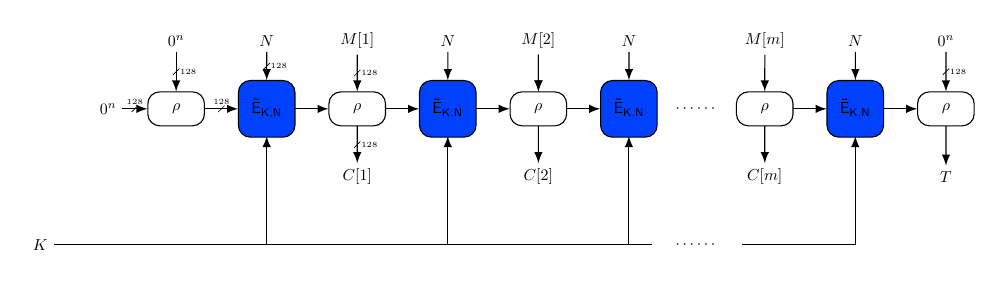
\begin{tikzpicture}[scale=0.575, every node/.style={transform shape}]
        \node (key) at (-3, -3) {$K$};
        \draw (-2.7, -3) -- (10.5, -3);
        \draw [-latex] (10,-3) -- (10, -0.6);
        \draw [-latex] (2,-3) -- (2, -0.6);
        \draw [-latex] (6,-3) -- (6, -0.6);
        \draw (12.5, -3) -- (15, -3);
        \draw [-latex] (15,-3) -- (15, -0.6);
        \node at (11.5,-3) {$\cdots\cdots$};

        \node (r0) at (0,0) [minimum size=1.25cm, minimum height = 0.75cm, rounded corners=1ex, draw] {$\rho$};
        \node (0) [above of=r0, node distance = 1.5cm] {$0^n$};
        \node (00) [left of=r0, node distance = 1.5cm] {$0^n$};
        \draw[next] (0) -- node {\bitwidth} node[bitwidthvert] {$128$} (r0);            
        \draw[next] (00) -- node {\bitwidth} node[bitwidth] {$128$} (r0);            

        \draw (2,0) \tencdpa{enc1};

        %\node (E1) [fill = blue!80, right of=r0, node distance=2cm, minimum size=1.25cm,rounded corners=1ex, draw] { $\tilde{E}_K^{26, 0}$};
        \node (n1) [above of=enc1, node distance = 1.5cm] {$N$};
        \draw[next] (n1) -- node {\bitwidth} node[bitwidthvert] {$128$} (enc1);            
        
        \draw[next] (r0) -- node {\bitwidth} node[bitwidth] {$128$} (enc1);            

        \node (r1) [right of=enc1, node distance=2cm, minimum size=1.25cm, minimum height = 0.75cm, rounded corners=1ex, draw] {$\rho$};
        \node (M1) [above of=r1, node distance = 1.5cm] {$M[1]$};
        \node (C1) [below of=r1, node distance = 1.5cm] {$C[1]$};

        \draw[-latex] (enc1) -- (r1);
        \draw[next] (M1) -- node {\bitwidth} node[bitwidthvert] {$128$} (r1);            
        \draw[next] (r1) -- node {\bitwidth} node[bitwidthvert] {$128$} (C1);            

        \draw (6,0) \tencdpa{enc2};
        \node (n2) [above of=enc2, node distance = 1.5cm] {$N$};
        \draw[-latex] (n2) -- (enc2);


        \draw[-latex] (r1) -- (enc2);
        \node (r2) [right of=enc2, node distance=2cm, minimum size=1.25cm, minimum height = 0.75cm, rounded corners=1ex, draw] {$\rho$};
        \node (M2) [above of=r2, node distance = 1.5cm] {$M[2]$};
        \node (C2) [below of=r2, node distance = 1.5cm] {$C[2]$};
        \draw[-latex] (enc2) -- (r2);
        \draw[-latex] (r2) -- (C2);
        \draw[-latex] (M2) -- (r2);

        \draw (10,0) \tencdpa{enc3};
        \draw[-latex] (r2) -- (enc3);
        \node (n3) [above of=enc3, node distance = 1.5cm] {$N$};
        \draw[-latex] (n3) -- (enc3);

        \begin{scope}
            \node at (11.5,0) {$\cdots\cdots$};
        \end{scope}
                    \draw[-latex] (M2) -- (r2);

        \node (r3) at (13,0) [minimum size=1.25cm, minimum height = 0.75cm, rounded corners=1ex, draw] {$\rho$};
        \node (Mm) [above of=r3, node distance = 1.5cm] {$M[m]$};
        \node (Cm) [below of=r3, node distance = 1.5cm] {$C[m]$};
        \draw[-latex] (r3) -- (Cm);
        \draw[-latex] (Mm) -- (r3);

        \draw (15,0) \tencdpa{E4};
        \node (n4) [above of=E4, node distance = 1.5cm] {$N$};
        \draw[-latex] (n4) -- (E4);
        \node (r4) [right of=E4, node distance=2cm, minimum size=1.25cm, minimum height = 0.75cm, rounded corners=1ex, draw] {$\rho$};
        \draw[-latex] (r3) -- (E4);
        \draw[-latex] (E4) -- (r4);

        \node (000) [above of=r4, node distance = 1.5cm] {$0^n$};
        \draw[next] (000) -- node {\bitwidth} node[bitwidthvert] {$128$} (r4);            
        \node (T) [below of=r4, node distance = 1.5cm] {$T$};
        \draw[-latex] (r4) -- (T);


    % PARENTHESING
                

    %\node (r) at (2,5cm, 0) [minimum size=1.5cm, minimum height=0.75cm, rounded corners=1ex, draw] {{$\rho$}};
    %\node (0) [above of=r, node distance=2.5cm] {$0^n$};
    %\node (00) [left of=r, node distance = 2.5cm] {$0^n$};
    %\draw[-latex] (0) -- (r);
    %\draw[-latex] (00) -- (r);


    %\node (enc_init) [right of=r, node distance = 2.5cm, minimum size = 2cm, rounded corners=1ex,fill=blue!20,draw] {{\sc $\tilde{E}_K$}};
    %\draw[-latex] (r) -- (enc_init);

\end{tikzpicture}


	\caption{Uniformly protected implementation of Romulus-N (integrity with encryption leakage).
	Blue blocks have to be secure against DPA.}
        \label{fig:romulus_n}\vspace*{-0.5cm}
\end{figure}

\subsubsection{Grade-1 designs (internal re-keying).} A first step towards
building modes of operation that cope better with leakage is to embed an internal
re-keying mechanism. In this case, the mode first generates a fresh
key $K^*$ from the long-term key and the nonce, which is then updated 
after the processing of each message block. As a result, and 
as long as the adversary can only observe encryption leakage 
without nonce misuse, only the KDF needs security against DPA (as there is
a DPA using the nonce) and all the other computations must only be protected 
against SPA. Such a leveled implementation is illustrated in Figure~\ref{fig:photon}
for PHOTON-Beetle. Unfortunately, this guarantee vanishes
as soon as nonce misuse or decryption leakage are granted to the adversary.
In this case the adversary can target the processing of one message block
with many different messages (while keeping the nonce and all the the other message blocks constant)
and perform a DPA to recover the corresponding intermediate state. In the
case of a P-sponge construction~\cite{Sponge07}, it is then possible to invert the permutation
and get back to the long-term key. 
In the NIST lightweight
crypto competition, it is the case of 
PHOTON-Beetle, Sparkle and Xoodyak.

\begin{figure}
    \centering
    \input{./figures/mode_level_analysis/photon_CIL1.tex}
	\caption{Leveled implementation of PHOTON-Beetle (integrity with encryption leakage).
	Blue (resp., green) blocks have to be secure against DPA (resp., SPA).}
        \label{fig:photon}\vspace*{-0.5cm}
\end{figure}

\subsubsection{Grade-2 (Grade-1 + strengthened KDF/TGF).}
The second step towards
building modes of operation that cope better with leakage is to strengthen the
KDF/TGF so that the recovery of an internal state of the mode cannot
lead to long-term secrets. This is easily (and efficiently) done
by making the KDF and the TGF non-invertible. In the case of 
sponges, it can be achieved by XORing the long-term key before and
after the permutation used to generate the fresh key $K^*$ and the
tag $T$. For TBCs, it is a direct consequence of their PRP 
security. In the NIST lightweight
crypto competition, it is for example the case of 
Ascon. For illustration, its leveled implementation 
is illustrated in
Figure~\ref{fig:Ascon}.

\begin{figure}[h]
    \begin{subfigure}{\textwidth} \centering
	\input{figures/mode_level_analysis/ascon_CIL1.tex}\caption{Integrity requirements (with decryption leakage).}
	\end{subfigure}
	\begin{subfigure}{\textwidth} \centering
	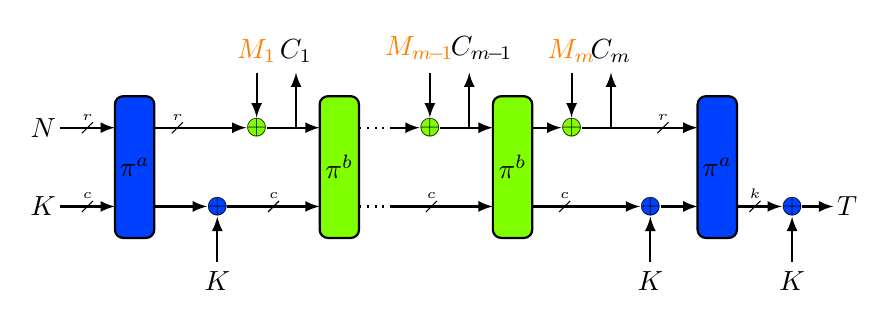
\begin{tikzpicture}[thick]
  % --- init up to p^a ---
  \begin{scope}[xshift=0cm]
      \draw (0,\rate) node[left, sparsam] {$N$};
      \draw (0,-\rate) node[left, sparsam] {$K$};

      \draw[next] (0,\rate) -- node {\bitwidth} node[bitwidth] {$r$} (.7,\rate);
      \draw[next] (0,-\rate) -- node {\bitwidth} node[bitwidth] {$c$} (.7,-\rate);



    \draw (.95,0) \permdpa{a};
  \end{scope}

  % --- enc P1 ---
  \begin{scope}[xshift=1.2cm]
    \draw (.8,-\rate) \xordpa{AuthPad};
    \draw[next] (0,-\rate) -- (AuthPad);
    \draw[next] (AuthPad) +(0,-\msg) node[below] {$K$} -- (AuthPad);
    \draw[next] (AuthPad) -- node {\bitwidth} node [bitwidth] {$c$} +(1.3, 0);

    %\draw[dashdotted] (.8,1.5) -- (.8,-1.5);

    \draw (1.3,\rate) \xorspa{P1};
    \draw[next] (0,\rate) -- node[near start] {\bitwidth} node[near start, bitwidth] {$r$} (P1);
    \draw[next] (P1) +(0,\msg) node[above, color = orange] {$M_1$} -- (P1);
    \draw[next] (P1) -- +(2*\minnext,0);
    \draw[next] (P1) ++(.5,0) -- +(0,\msg) node[above] {$C_1$};

    \draw (2.35,0) \permspa{b};
  \end{scope}

  % --- enc Pt-1 ---
  \begin{scope}[xshift=3.8cm]
    \draw[dotted] (0,\rate) -- (\minnext,\rate)
                  (0,-\rate) -- (\minnext,-\rate);

    \draw[next] (\minnext,-\rate) -- node[pos=.4] {\bitwidth} node [pos=.4,bitwidth] {$c$} +(1.3,0);

    \draw (.9,\rate) \xorspa{Pt1};
    \draw[next] (\minnext,\rate) -- (Pt1);
    \draw[next] (Pt1) +(0,\msg) node[above, color = orange] {$M_{m\!-\!1}$ \hspace*{.15cm}} -- (Pt1);
    \draw[next] (Pt1) -- +(.8,0);
    \draw[next] (Pt1) ++(.5,0) -- +(0,\msg) node[above] {\hspace*{.2cm} $C_{m\!-\!1}$};

    \draw (1.95,0) \permspa{b};
  \end{scope}

  % --- enc Pt and finalize ---
  \begin{scope}[xshift=6.0cm]
    \draw (.5,\rate) \xorspa{Pt};
    \draw[next] (0,\rate) -- (Pt);
    \draw[next] (Pt) +(0,\msg) node[above, color = orange] {$M_m$} -- (Pt);
    \draw[next] (Pt) ++(.5,0) -- +(0,\msg) node[above] {$C_m$};
    \draw[next] (Pt) -- node[pos=.7] {\bitwidth} node[pos=.7,bitwidth] {$r$} +(1.6,0);

    %\draw[dashdotted] (1.3,1.5) -- (1.3,-1.5);

    \draw (1.5,-\rate) \xordpa{Kf};
    \draw[next] (Kf) +(0,-\msg) node[below] {$K$} -- (Kf);
    \draw[next] (0,-\rate) -- node[pos=.3] {\bitwidth} node[pos=.3,bitwidth] {$c$} (Kf);
    \draw[next] (Kf) -- (2.1,-\rate);

    \draw (2.35,0) \permdpa{a};

    \draw (3.3,-\rate) \xordpa{Kt};
    \draw[next] (Kt) +(0,-\msg) node[below] {$K$} -- (Kt);
    \draw[next] (2.6,-\rate) -- node[pos=.4] {\bitwidth} node[pos=.4,bitwidth] {$k$} (Kt);
    \draw (4.0,-\rate) node[name=T,sparsam] {$T$};
    \draw[next] (Kt) -- (T);
  \end{scope}

\end{tikzpicture}\caption{Confidentiality requirements (without decryption leakage).}
	\end{subfigure}
        \caption{Leveled implementation of Ascon.
            The blue blocks have to be protected against DPA and the green blocks
            have to be protected against SPA, while the white ones do not require
            protection against side-channel leakage.
        }
        \label{fig:Ascon}
\end{figure}

\medskip

The top of the figure depicts the integrity requirements. In this case, only
the KDF and the TGF (in blue) must be protected against DPA  and the rest of the computations (in white)
can leak in full. This guarantee holds even when nonce misuse and
leakage in decryption are granted to the adversary. It intuitively derives
from the fact that the ephemeral secrets cannot be used to infer long-term ones,
and corresponds to the top of the hierarchy introduced in~\cite{DBLP:conf/latincrypt/GuoPPS19}.
The bottom of the figure 
depicts the confidentiality requirements. In this case, it is naturally 
not possible to tolerate unbounded leakage. Yet, as long as the adversary 
is not granted with decryption leakage, only SPA security (in green) is required 
for this part of the computation. (The orange color for the plaintexts
is used to reflect that even their very manipulation may leak sensitive information).
The main attack vector that remains against this construction happens
with decryption leakage. Since the message is decrypted before
verifying the tag, an adversary can then 
target the processing of one message block with many different
messages (keeping the nonce and all the the other message blocks constant) and perform
a DPA to recover the corresponding intermediate state.
This reveals the ephemeral keystream, hence the message, but does not
affect the confidentiality of messages encrypted with a different nonce.

\subsubsection{Grade-3 (Grade-2 + two passes).}
The natural way to get rid of the last attack vector against Ascon
is to consider 2-pass designs (such as encrypt-then-MAC constructions).
In this case, the tag can be computed
from the ciphertext blocks and tested before the decryption takes place. 
 In the NIST lightweight
crypto competition, it is for example the case of 
ISAP (which is permutation-based) and Romulus-T (which is TBC-based). 
Their main difference lies in the way they secure their KDF and TGF.
Like Ascon,
Romulus-T (which is based on the TEDT mode of operation~\cite{DBLP:journals/tches/BertiGPPS20})
relies on masking for this purpose. By contrast, ISAP relies on 
a leakage-resilient PRF. As illustrated in Figure~\ref{fig:ISAP}, the leakage-resilient PRF
can be viewed as a re-keying scheme where the nonce bits are absorbed one 
by one so that each of its intermediate keys is only used to process two 
permutation calls. As a result, this PRF essentially ``reduces'' DPA security to SPA 
security, at the cost of iterating the Ascon-p$^1$ permutation.\footnote{Increasing the rate 
to absorb more bits and get a more efficient design is possible but it then opens
a DPA attack vector (so we do not consider this option here).}

\begin{figure}
    \centering
    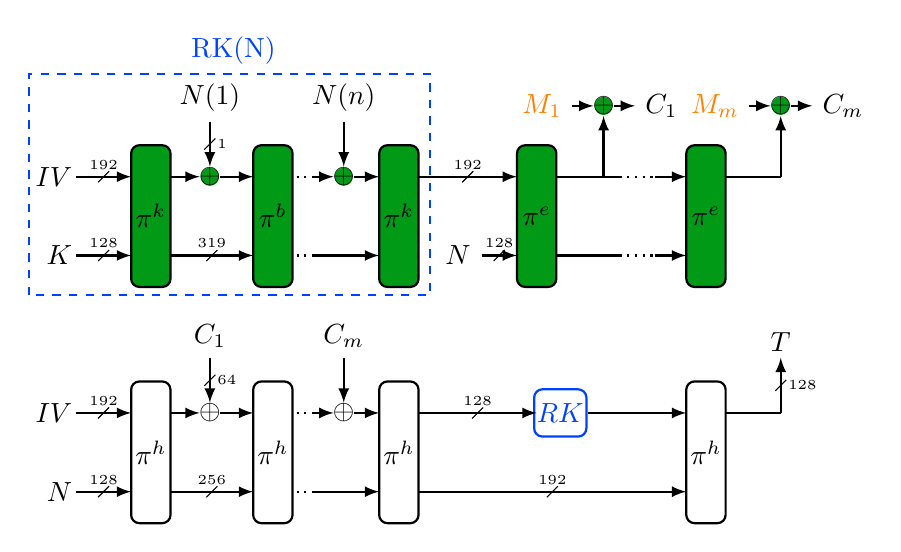
\begin{tikzpicture}[thick]

    % Draw RK box
    \draw [color = DPAblue] (2,2.1) node {RK(N)};
	\draw[thick,dashed, color = DPAblue] (-0.6, -1) rectangle ++(5.1,2.8);
  % --- init with IV, K ---
  \begin{scope}[xshift=0cm]
      \draw (0,\rate) node[left, sparsam] {$IV$};
      \draw (0,-\rate) node[left, sparsam] {$K$};

      \draw[next] (0,\rate) -- node {\bitwidth} node[bitwidth] {$192$} (.7,\rate);
      \draw[next] (0,-\rate) -- node {\bitwidth} node[bitwidth] {$128$} (.7,-\rate);

      \draw (.95,0) \permspav{k};
  \end{scope}

  % --- absorb N1 ---
  \begin{scope}[xshift=1cm]
    \draw[next] (0.2, -\rate) -- node {\bitwidth} node [bitwidth] {$319$} +(1.05,0);

    %\draw[dashdotted] (.8,1.5) -- (.8,-1.5);

    \draw (0.7,\rate) \xorspav{N1};
    \draw[-latex] (0.2,\rate) -- (N1);
    \draw[next] (N1) +(0,\msg) node[above] {$N(1)$} -- node {\bitwidth} node[bitwidthvert] {$1$} (N1);
    \draw[next] (N1) -- +(0.55,0);

    \draw (1.5,0) \permspav{b};
  \end{scope}

  % --- absorb Nn ---
  \begin{scope}[xshift=2.6cm]
    \draw[dotted] (0.2,\rate) -- (\minnext,\rate)
                  (0.2,-\rate) -- (\minnext,-\rate);

    \draw (.8,\rate) \xorspav{Nn};
    \draw[next] (\minnext,\rate) -- (Nn);
    \draw[next] (Nn) +(0,\msg) node[above] {$N(n)$} -- (Nn);
    \draw[next] (Nn) -- +(0.45,0);

    \draw[-latex] (\minnext,-\rate) -- (1.25,-\rate);

    \draw (1.5,0) \permspav{k};
  \end{scope}

  % --- Finish nonce absorption ---
  \begin{scope}[xshift=4.35cm]
  
    \draw (0.5, -\rate) node {$N$};
    \draw[next] (0.8,-\rate) -- node {\bitwidth} node[bitwidth] {$128$} (1.25, -\rate);

    %\draw[dashdotted] (.8,1.5) -- (.8,-1.5);

    \draw[next] (0,\rate) -- node{\bitwidth} node [bitwidth] {$192$} (1.25, \rate);

    \draw (1.5,0) \permspav{e};
  \end{scope}

  % --- enc M1 ---
  \begin{scope}[xshift=6.1cm]
    \draw (0,-\rate) -- (0.8, -\rate);

    \draw (0,\rate) -- (0.8, \rate);
    
    \draw (0.6, 1.4) \xorspav{Pt1};
    \draw[next] (0.6,\rate) -- (Pt1);
    \draw[next] (Pt1) +(-0.4, 0) node[left, color = orange] {$M_{1}$} -- (Pt1);
    \draw[next] (Pt1) -- +(0.4,0) node[right] {$C_{1}$};
    
    \draw[dotted] (0.8,\rate) -- (1.25,\rate)
                  (0.8,-\rate) -- (1.25,-\rate);
                  
    \draw[next] (1.25,-\rate) -- (1.65, -\rate);
    \draw[next] (1.25,\rate) -- (1.65, \rate);
    
    \draw (1.9,0) \permspav{e};
  \end{scope}

  % --- enc Mm ---
  \begin{scope}[xshift=8.25cm]

    \draw (0.7, 1.4) \xorspav{Pt1};
    \draw[next] (0.7,\rate) -- (Pt1);
    \draw (0, \rate) -- (0.7, \rate);
    \draw[next] (Pt1) +(-0.4, 0) node[left, color = orange] {$M_{m}$} -- (Pt1);
    \draw[next] (Pt1) -- +(0.4,0) node[right] {$C_{m}$};
  \end{scope}

    \begin{scope}[yshift=-3cm, xshift = 0cm]
      \draw (0,\rate) node[left, sparsam] {$IV$};
      \draw (0,-\rate) node[left, sparsam] {$N$};

      \draw[next] (0,\rate) -- node {\bitwidth} node[bitwidth] {$192$} (.7,\rate);
      \draw[next] (0,-\rate) -- node {\bitwidth} node[bitwidth] {$128$} (.7,-\rate);

      \draw (.95,0) \perm{h};

    \end{scope}
  \begin{scope}[yshift = -3cm, xshift=1cm]
    \draw[next] (0.2, -\rate) -- node {\bitwidth} node [bitwidth] {$256$} +(1.05,0);

    %\draw[dashdotted] (.8,1.5) -- (.8,-1.5);

    \draw (0.7,\rate) \xor{N1};
    \draw[-latex] (0.2,\rate) -- (N1);
    \draw[next] (N1) +(0,\msg) node[above] {$C_1$} -- node {\bitwidth} node[bitwidthvert] {$64$} (N1);
    \draw[next] (N1) -- +(0.55,0);

    \draw (1.5,0) \perm{h};
  \end{scope}
  
    \begin{scope}[yshift = -3cm, xshift=2.6cm]
    \draw[dotted] (0.2,\rate) -- (\minnext,\rate)
                  (0.2,-\rate) -- (\minnext,-\rate);

    \draw (.8,\rate) \xor{Nn};
    \draw[next] (\minnext,\rate) -- (Nn);
    \draw[next] (Nn) +(0,\msg) node[above] {$C_m$} -- (Nn);
    \draw[next] (Nn) -- +(0.45,0);

    \draw[-latex] (\minnext,-\rate) -- (1.25,-\rate);

    \draw (1.5,0) \perm{h};
  \end{scope}
  \begin{scope}[yshift = -3cm, xshift=4.35cm]

    %\draw[dashdotted] (.8,1.5) -- (.8,-1.5);
    
    \draw (1.8, \rate) node [rectangle, rounded corners=3pt, minimum width=.5cm, minimum height=.6cm, draw, sparsam, color = DPAblue] {$RK$};
    
    \draw[next] (0, \rate) -- node{\bitwidth} node [bitwidth] {$128$} (1.5, \rate);
    \draw[next] (0, -\rate) -- node{\bitwidth} node [bitwidth] {$192$} (3.4, -\rate);

  \end{scope}
  \begin{scope}[yshift=-3cm, xshift=6.1cm]
  
    \draw[next] (.4,\rate) -- (1.65, \rate);
    
    \draw (1.9,0) \perm{h};
  \end{scope}
  \begin{scope}[yshift=-3cm, xshift=8.25cm]
    \draw (0,\rate) -- (0.7, \rate);
    \draw[next] (0.7,\rate) -- node {\bitwidth} node [bitwidthvert] {$128$} (0.7, 1.2);
    \draw (0.7, 1.4)  node {$T$};
  \end{scope}

\end{tikzpicture}
	\caption{
            Leveled implementation of ISAP (confidentiality with decryption leakage).
            The green blocks have to be protected against SPA (with averaging), while the white
            ones do not require any protection against side-channel leakage.
        }\label{fig:ISAP}
\end{figure}

\begin{figure}
    \centering
    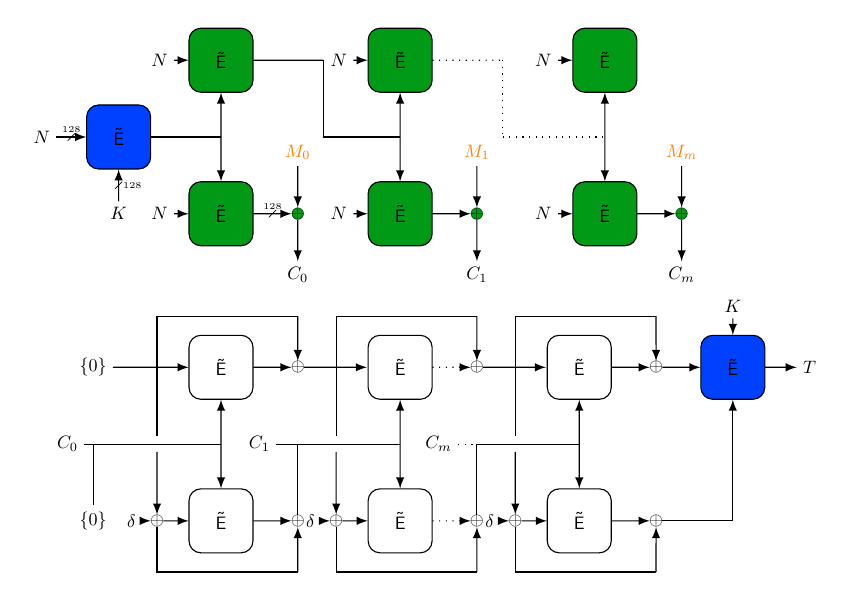
\begin{tikzpicture}[scale=0.65, every node/.style={transform shape}]

    \draw (1,0) \tbcdpa{enc1};
    \node (n) [left of=enc1, node distance = 1.5cm] {$N$};
    \node (k) [below of=enc1, node distance = 1.5cm] {$K$};
    \draw[next] (n) -- node {\bitwidth} node[bitwidth] {$128$} (enc1);            
    \draw[next] (k) -- node {\bitwidth} node[bitwidthvert] {$128$} (enc1); 
    \draw[] (enc1) -- (3,0);            
           
    \begin{scope}[xshift=0cm]
        \draw (3,1.5) \tbcspav{enc2};
        \node (n) [left of=enc2, node distance = 1.2cm] {$N$};
        \draw[next] (n) -- (enc2);            

        \draw (3,-1.5) \tbcspav{enc3};
        \node (n2) [left of=enc3, node distance = 1.2cm] {$N$};
        \draw[next] (n2) -- (enc3);            

        \draw (4.5, -1.5) \xorspav{m0};
        \node (m) [above of=m0, node distance = 1.2cm, color = orange] {$M_0$};
        \node (c) [below of=m0, node distance = 1.2cm] {$C_0$};
        \draw[next] (enc3) -- node {\bitwidth} node[bitwidth] {$128$} (m0);            
        \draw[next] (m) -- (m0);            
        \draw[next] (m0) -- (c);            
        \draw[next] (3, 0) -- (enc2);            
        \draw[next] (3, 0) -- (enc3); 
        \draw[] (enc2) -- (5,1.5);            
        \draw[] (5,1.5) -- (5, 0);            
        \draw[] (5,0) -- (6.5, 0);            
      
    \end{scope}
    \begin{scope}[xshift=3.5cm]
        \draw (3,1.5) \tbcspav{enc2};
        \node (n) [left of=enc2, node distance = 1.2cm] {$N$};
        \draw[next] (n) -- (enc2);            

        \draw (3,-1.5) \tbcspav{enc3};
        \node (n2) [left of=enc3, node distance = 1.2cm] {$N$};
        \draw[next] (n2) -- (enc3); 
        \draw (4.5, -1.5) \xorspav{m0};
        \node (m) [above of=m0, node distance = 1.2cm, color = orange] {$M_1$};
        \node (c) [below of=m0, node distance = 1.2cm] {$C_1$};
        \draw[next] (enc3) -- (m0);            
        \draw[next] (m) -- (m0);            
        \draw[next] (m0) -- (c);            
        \draw[next] (3, 0) -- (enc2);            
        \draw[next] (3, 0) -- (enc3); 
        \draw[dotted] (enc2) -- (5,1.5);            
        \draw[dotted] (5,1.5) -- (5, 0);            
        \draw[dotted] (5,0) -- (7, 0);            
      
    \end{scope}
    \begin{scope}[xshift=7.5cm]
        \draw (3,1.5) \tbcspav{enc2};
        \node (n) [left of=enc2, node distance = 1.2cm] {$N$};
        \draw[next] (n) -- (enc2);            

        \draw (3,-1.5) \tbcspav{enc3};
        \node (n2) [left of=enc3, node distance = 1.2cm] {$N$};
        \draw[next] (n2) -- (enc3); 
        \draw (4.5, -1.5) \xorspav{m0};
        \node (m) [above of=m0, node distance = 1.2cm, color = orange] {$M_m$};
        \node (c) [below of=m0, node distance = 1.2cm] {$C_m$};
        \draw[next] (enc3) -- (m0);            
        \draw[next] (m) -- (m0);            
        \draw[next] (m0) -- (c);            
        \draw[next] (3, 0) -- (enc2);            
        \draw[next] (3, 0) -- (enc3); 
    \end{scope}

    \begin{scope}[xshift=0cm, yshift = -6cm]
        \draw (3,1.5) \tbc{enc2};
        \node (L) [left of=enc2, node distance = 2.5cm] {$\{0\}$};
        \node (C) at (0,0) [] {$C_0$};
        \node (R) at (.5,-1.5) [] {$\{0\}$};
        \draw[] (R) |- (3, 0);            
        \draw[] (C) -- (3, 0);            

        \draw[next] (L) -- (enc2);            

        \draw (3,-1.5) \tbc{enc3};
        \draw (1.75, -1.5) \xor{deltax};
        \node (delta) [left of=deltax, node distance = .5cm] {$\delta$};

        \draw[next] (deltax) -- (enc3);            
        \draw[next] (delta) -- (deltax);   
        \draw[] (1.75,1.5) -- (1.75,.15);                     
        \draw[next] (1.75,-.15) -- (deltax);            

        \draw[] (1,0) -- (3,0);            
        \draw[next] (3,0) -- (enc3);            
        \draw[next] (3,0) -- (enc2);            

        \draw (4.5, 1.5) \xor{deltat};
        \draw[next] (enc2) -- (deltat);            
        \draw[] (1.75,1.5) |- (4.5, 2.5);            
        \draw[next] (4.5,2.5) -- (deltat);            
        \draw[next] (deltat) -- (5.85,1.5);            

        \draw (4.5, -1.5) \xor{deltat2};
        \draw[next] (enc3) -- (deltat2);            
        \draw[] (deltax) |- (4.5, -2.5);            
        \draw[next] (4.5,-2.5) -- (deltat2);            
        \draw[] (deltat2) |- (5,0);            



    \end{scope}

    \begin{scope}[xshift=3.5cm, yshift = -6cm]
        \draw (3,1.5) \tbc{enc2};
        \node (C) at (0.25,0) [] {$C_1$};
        \draw[] (deltat2) |- (3, 0);            
        \draw[] (C) -- (3, 0);            


        \draw (3,-1.5) \tbc{enc3};
        \draw (1.75, -1.5) \xor{deltax};
        \node (delta) [left of=deltax, node distance = .5cm] {$\delta$};

        \draw[next] (deltax) -- (enc3);            
        \draw[next] (delta) -- (deltax);   
        \draw[] (1.75,1.5) -- (1.75,.15);                     
        \draw[next] (1.75,-.15) -- (deltax);            

        \draw[] (1,0) -- (3,0);            
        \draw[next] (3,0) -- (enc3);            
        \draw[next] (3,0) -- (enc2);            

        \draw (4.5, 1.5) \xor{deltat};
        \draw[next, dotted] (enc2) -- (deltat);            
        \draw[] (1.75,1.5) |- (4.5, 2.5);            
        \draw[next] (4.5,2.5) -- (deltat);            
        \draw[next] (deltat) -- (5.85,1.5);            

        \draw (4.5, -1.5) \xor{deltat2};
        \draw[next, dotted] (enc3) -- (deltat2);            
        \draw[] (deltax) |- (4.5, -2.5);            
        \draw[next] (4.5,-2.5) -- (deltat2);            
        \draw[] (deltat2) |- (5,0);            

    \end{scope}
    \begin{scope}[xshift=7cm, yshift = -6cm]
        \draw (3,1.5) \tbc{enc2};

        \draw (3,-1.5) \tbc{enc3};
        \draw (1.75, -1.5) \xor{deltax};
        \node (delta) [left of=deltax, node distance = .5cm] {$\delta$};
        \draw (6,1.5) \tbcdpa{enc4};


        \draw[next] (deltax) -- (enc3);            
        \draw[next] (delta) -- (deltax);   
        \draw[] (1.75,1.5) -- (1.75,.15);                     
        \draw[next] (1.75,-.15) -- (deltax);            

        \draw[] (1,0) -- (3,0);            
        \draw[next] (3,0) -- (enc3);            
        \draw[next] (3,0) -- (enc2);            

        \draw (4.5, 1.5) \xor{deltat};
        \draw[next] (enc2) -- (deltat);            
        \draw[] (1.75,1.5) |- (4.5, 2.5);            
        \draw[next] (4.5,2.5) -- (deltat);            
        \draw[next] (deltat) -- (enc4);            

        \draw (4.5, -1.5) \xor{deltat2};
        \draw[next] (enc3) -- (deltat2);            
        \draw[] (deltax) |- (4.5, -2.5);            
        \draw[next] (4.5,-2.5) -- (deltat2);            
        \draw[next] (deltat2) -| (enc4);         

        \node (tag) [right of=enc4, node distance = 1.5cm] {$T$};
        \draw[next] (enc4) -- (tag);            
        \node (key) [above of=enc4, node distance = 1.2cm] {$K$};
        \draw[next] (key) -- (enc4);            

        \node (C) at (0.25,0) [] {$C_m$};
        \draw[dotted] (C) -- (3, 0);            


    \end{scope}
\end{tikzpicture}
    \caption{Leveled implementation of Romulus-T (confidentiality with decryption leakage).
            The blue blocks have to be protected against DPA and the green blocks
            have to be protected against SPA (with averaging), while the white ones do not require any
            protection against side-channel leakage.
    }
    \label{fig:TEDT}
\end{figure}

Overall, ISAP's confidentiality with decryption leakage requires two calls to the
leakage-resilient PRF and a plaintext processing that is secure against SPA.
We provide a similar picture for the leveled implementation
of Romulus-T in Figure~\ref{fig:TEDT}, where the KDF and TGF
are directly instantiated with a masked TBC. 
Note that the SPA-secure blocks of these two figures are in dark green to reflect the possibility
that the adversary repeats the same measurements to average the noise.
And as in the case of Ascon,
integrity with decryption leakage only requires the two protected calls (to 
the leakage-resilient PRF or masked TBC) and can let all the other computations leak in full.



\section{Hardware implementations}\label{sec:implem}

Given the previous analysis, it appears that Ascon, ISAP and Romulus-T are
the most promising candidates of the NIST lightweight crypto competition
for leakage-resistant implementations. In this section, we therefore investigate
their hardware implementations. For this purpose, we focus on
the security guarantees that they enable without a uniformly protected implementation.
We first investigate their primitives, with a special focus on Romulus-T
and its underlying TBC Skinny-384+ (for which, as mentioned in introduction,
the literature is a bit scarcer). We then detail the implementation of the
modes and report their performances (with ASIC synthesis). We use these results to confirm the
relevance of leveled implementations and to discuss the respective interest
of the three implemented ciphers in the context of the NIST competition.

\subsection{Masked implementation of the primitives}\label{subsec:prim}

We use the HPC2 masking scheme, as it allows almost arbitrary composition while
ensuring security against both hardware glitches and
transitions~\cite{DBLP:journals/tc/CassiersGLS21,DBLP:journals/tches/CassiersS21}.
The main characteristics of this masking scheme are the following.
The linear operations are very efficient, since they are made of purely
combinational logic and have a linear overhead in the masking order.
On the other hand, the non-linear operation, which is the 2-input AND gate (see
\autoref{algo:hpc2_mul}), has quadratic
overhead and asymmetric latency: 2~cycles with respect to one input, and only
1~cycle with respect to the other input.

\begin{algorithm}[tb]
    \caption{HPC2 AND gadget with $\nShares$ shares (sync. registers
    are omitted).}
    \label{algo:hpc2_mul}
    \begin{algorithmic}[1]
        \Require Sharings $\sharing{x}$, $\sharing{y}$
        \Ensure Sharing $\sharing{z}$ such that $z = x \cdot y$.
        \algrule
        \For{$i = 0 \text{ to }d-1$}
            \For{$j = i+1 \text{ to }d-1$}
                \State $r_{ij} \randtake \ft; \ r_{ji} \gets r_{ij}$
            \EndFor
        \EndFor
        \For{$i = 0 \text{ to }d-1$}
            \State $\share{z}{i} \gets \share{x}{i}\share{y}{i}$
            \For{$j = 0 \text{ to }d-1, j\neq i$}
                \State $\share{z}{i} \gets
                \share{z}{i} \oplus
                    \func{\reg}{\left(\share{x}{i}\oplus 1\right) r_{ij}}
                    \oplus \func{\reg}{\share{x}{i}\func{\reg}{\share{y}{j}\oplus r_{ij}}}
                    $
            \EndFor
        \EndFor
    \end{algorithmic}
\end{algorithm}


\subsubsection{Skinny Sbox.}\label{subsub:skinny_sbox}
The Skinny Sbox (depicted in \autoref{fig:sboxclean}) is made of XOR gates (that are
linear, and therefore easy to implement) and of NOR gates that we implement
with a AND gate whose inputs are inverted.

We next propose two area-optimized architectures for this Sbox, that both
instantiate two masked AND and two masked XOR gates.
\begin{figure}
    \centering
    \input{figures/implem_prim/sbox_skinny.tex}
    \caption{Skinny Sbox circuit representation with NOR and XOR gates.}
    \label{fig:sboxclean}
\end{figure}
First, the high-throughput one is based on the observation that the Sbox can be
decomposed into 4~applications of a simpler function (as visible in
\autoref{fig:sboxclean}), followed by a wire shuffling.
This function has a latency of at least two cycles with our masking
scheme, due to the AND gate.
We therefore build the high-throughput Sbox by looping 4~times on a two-stage
pipeline.
The core of this pipeline is a simple function block B shown in
\autoref{fig:block}, which is then used twice and connected to combinational
logic to form the Sbox (\autoref{fig:sboxser_circuit}).
The two-stage pipeline can be used to perform simultaneously two Sbox
operations.
We finally add input and output synchronization registers such that the logic
performs two Sbox evaluations in 9~clock cycles, without the need for any
external synchronization mechanism.
\begin{figure}
	\begin{subfigure}[b]{.48\textwidth}
		\centering
		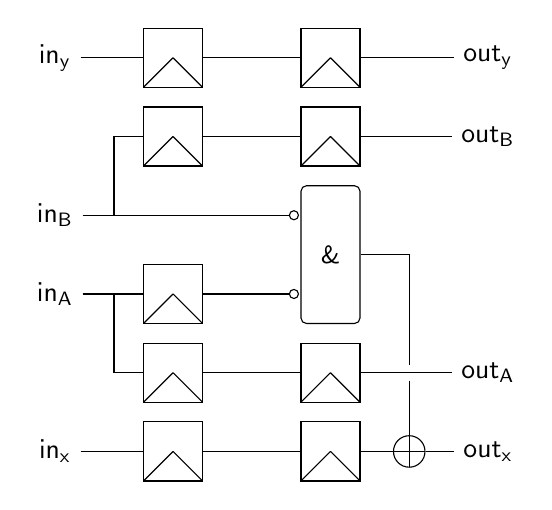
\begin{tikzpicture}[]
  %\draw [] (0, 0) \register{reg1};
  \draw [] (0, 1) \register{reg1};
  \draw [] (2, 1) \register{reg2};
  \draw [] (0, 3) \register{reg3};
  \draw [] (0, 6) \register{reg4};
  \draw [] (2, 6) \register{reg5};
  \draw [] (0, 5) \register{reg6};
  \draw [] (2, 5) \register{reg7};
  \draw [] (0, 2) \register{reg8};
  \draw [] (2, 2) \register{reg9};

  \draw [] (3, 1) \xord{xor1};

  \node[rectangle,
  minimum width = .75cm,
  minimum height = 1.75cm,
  draw,
  rounded corners = 2pt
  ] (B2) at (2,3.5) {\small \textsf{\&}};

  \node [] (ina) at (-1.5, 3) {$\mathsf{in}_\mathsf{A}$};
  \node [] (inb) at (-1.5, 4) {$\mathsf{in}_\mathsf{B}$};
  \node [] (inx) at (-1.5, 1) {$\mathsf{in_x}$};
  \node [] (iny) at (-1.5, 6) {$\mathsf{in_y}$};

  \node [] (outx) at (4, 1) {$\mathsf{out_x}$};
  \node [] (outa) at (4, 2) {$\mathsf{out_A}$};
  \node [] (outb) at (4, 5) {$\mathsf{out_B}$};
  \node [] (outz) at (4, 6) {$\mathsf{out_y}$};

  \draw[] (iny) -- (reg4);
  \draw[] (reg4) -- (reg5);
  \draw[] (reg5) -- (outz);

  \draw[] (ina) -- (reg3);
  \draw[{-Circle[open]}] (inb) -- (1.6,4);
  \draw[{-Circle[open]}] (reg3) -- (1.6,3);
  \draw[] (inx) -- (reg1);
  \draw[] (reg1) -- (reg2);
  \draw[] (reg2) -- (xor1);
  \draw[] (B2) -| (3,2.1);
  \draw[] (3, 1.9) -- (xor1);
  \draw[] (xor1) -- (outx);

    \draw[] (-.75,4) -- (-.75, 5);
    \draw[] (-.75,5) -- (reg6);
    \draw[] (reg6) -- (reg7);
    \draw[] (reg7) -- (outb);

    \draw[] (-.75,3) -- (-.75, 2);
    \draw[] (-.75,2) -- (reg8);
    \draw[] (reg8) -- (reg9);
    \draw[] (reg9) -- (outa);

\end{tikzpicture}
		\caption{%
                    Inner logic block ``B'' for Sbox implementation, with one
                    AND and one XOR.
                }
                \label{fig:block}
	\end{subfigure}
        \hfill
	\begin{subfigure}[b]{.48\textwidth}
		\centering
		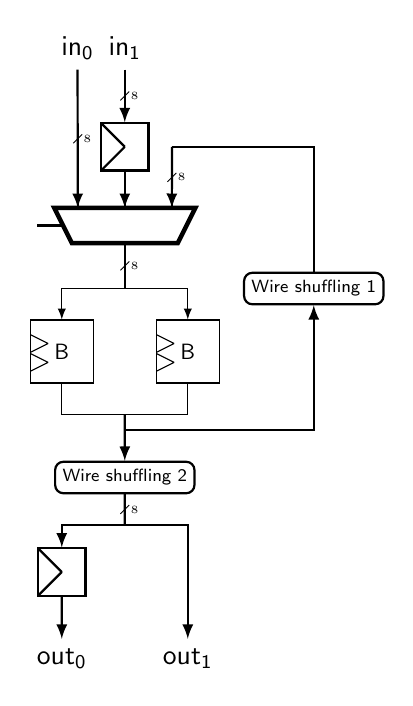
\begin{tikzpicture}[]
    \node [] (in1) at (-.6, 2.25) {$\mathsf{in_0}$};
    \node [] (in0) at (0, 2.25) {$\mathsf{in_1}$};
    \node [] (o1) at (-.8, -5.5) {$\mathsf{out_0}$};
    \node [] (o0) at (.8, -5.5) {$\mathsf{out_1}$};
\begin{scope}[scale=.8, every node/.style={transform shape}]
    
    \node[rectangle,
    latency,
    minimum width = 1cm,
    minimum height = 1cm,
    draw] (B1) at (-1,-2) {\textsf{B}};

    \draw [thick] (0, 1.25) \registerrot{reg1};
    \draw [thick] (-1, -5.5) \registerrot{reg2};

    \node[rectangle,
    latency,
    minimum width = 1cm,
    minimum height = 1cm,
    draw,
    ] (B2) at (1,-2) {\textsf{B}};

    \node [mux 3by2, rotate = 270, thick](M1) at (0, 0){};

    \node[rectangle,
    minimum width = 1cm,
    rounded corners = 3pt,
    thick,
    minimum height = .5cm,
    draw] (ws1) at (0, -4) {\footnotesize \textsf{Wire shuffling 2}};

    \node[rectangle,
    minimum width = 1cm,
    rounded corners = 3pt,
    thick,
    minimum height = .5cm,
    draw] (ws2) at (3,-1) {\footnotesize \textsf{Wire shuffling 1}};

    \draw [thick, -latex] (0, -3.25) -| (ws2);
    \draw [thick] (M1.brpin 1) -- node {\bitwidth} node [bitwidthvert] {8} (0, -1);
    \draw [-latex, thick] (reg1) -- (M1.blpin 2);
    \draw [-latex, thick] (in1) -- node {\bitwidth} node [bitwidthvert] {8} (M1.blpin 3);

    \draw [-latex, thick] (in0) -- node {\bitwidth} node [bitwidthvert] {8} (reg1);
    \draw [-latex] (0, -1) -| (B1);
    \draw [-latex] (0, -1) -| (B2);
    \draw [] (B1) |- (0, -3);
    \draw [] (B2) |- (0, -3);
    \draw [thick, -latex] (0, -3) -- (ws1);
    \draw [thick] (ws2) |- (.75,1.25);
    \draw [thick, -latex] (.75, 1.25) -- node {\bitwidth} node [bitwidthvert] {8} (M1.blpin 1);

    \draw [thick] (ws1) -- node {\bitwidth} node [bitwidthvert] {8} (0, -4.75);
    \draw [-latex, thick] (0,-4.75) -| (reg2);

    \draw [-latex, thick] (0, -4.75) -| (o0);
    \draw [-latex, thick] (reg2) -- (o1);
\end{scope}

\end{tikzpicture}
		\caption{%
                    High-throughput Sbox architecture with input and output
                    sync. registers.
                }
                \label{fig:sboxser_circuit}
	\end{subfigure}
	\caption{%
            High-throughput masked Skinny Sbox.
        }
        \label{fig:sboxintro}
\end{figure}
Second, we design a low-latency architecture with an ALU-style design: the Sbox
inputs are stored in a register, as well as the outputs, and the data fed to
the two AND-XOR blocks are selected from these states (and from the input
wires) when needed (see \autoref{fig:sboxopt_circuit}).
This flexible architecture allows to benefit from the asymmetric latency of the
HPC2 AND gadgets, leading to a latency of 6~cycles for one Sbox evaluation (see
\autoref{fig:sbox_opt}).

\begin{figure}
    \begin{subfigure}[b]{.48\textwidth}
        \centering
        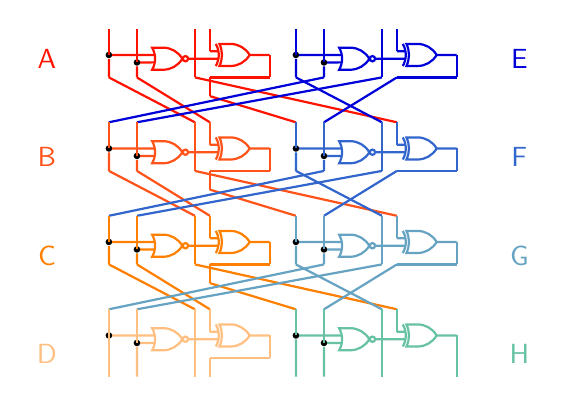
\begin{tikzpicture}[thick]
\begin{scope}
        
        \node [color = red!85!orange] (block1) at (-1.5, 0) {$\mathsf{A}$};
        \node [color = red!50!orange!90!white] (block2) at (-1.5, -1.25) {$\mathsf{B}$};
        \node [color = orange] (block3) at (-1.5, -2.5) {$\mathsf{C}$};
        \node [color = orange!50!white] (block1) at (-1.5, -3.75) {$\mathsf{D}$};
        \node [color = blue!85!black] (block1) at (4.5, 0) {$\mathsf{E}$};
        \node [color = blue!75!green!80!white] (block2) at (4.5, -1.25) {$\mathsf{F}$};
        \node [color = green!40!blue!60!white] (block3) at (4.5, -2.5) {$\mathsf{G}$};
        \node [color = green!60!blue!60!white] (block1) at (4.5, -3.75) {$\mathsf{H}$};

\end{scope}

        \begin{scope}[scale=0.475, every node/.style={transform shape}]
                
                \begin{scope}[yshift = 0cm]
                        \begin{scope}[color = red!85!orange]
                                \node[nor gate US, draw] at (0,0) (nor1) {};
                                \node[xor gate US, draw] at ($(nor1) + (1.8, 0.1)$) (xor1) {};
                                
                                \draw (nor1.output) -- (xor1.input 2);
                                \draw (-1.5, .1) -- (nor1.input 1);
                                \draw (-.75, -.1) -- (nor1.input 2);
                                \draw (1.2, .2) -- (xor1.input 1);
                                \draw (xor1.output) -- (2.8, .1);

                                \node[contact] (c1) at (-1.5,.1){};
                                \node[contact] (c2) at (-.75,-.1){};

                                % Input lines
                                \draw (-1.5,.8) -- (-1.5, .1);
                                \draw (-.75,.8) -- (-.75, -.1);
                                \draw (1.2, .8) -- (1.2, .2);
                                \draw (.8, .8) -- (.8, -.5);
                                % 1st input
                                \draw (c1) -- (-1.5, -.5);
                                \draw (-1.5, -.5) -- (.8, -1.7);
                                % 2nd input 
                                \draw (c2) -- (-.75, -.5);
                                \draw (-.75, -.5) -- (1.2, -1.7);
                                % 3rd input
                                \draw (.8, -.5) -- (6.2, -1.7);
                                % output
                                \draw (2.8,.1) -- (2.8, -.5);
                                \draw (2.8, -.5) -- (1.2, -.5);
                                \draw (1.2, -.5) -- (1.2, -1);
                                \draw (1.2, -1) -- (3.5, -1.7);


                        \end{scope}
                        \begin{scope}[xshift = 5cm, color = blue!85!black]
                                \node[nor gate US, draw] at (0,0) (nor1) {};
                                \node[xor gate US, draw] at ($(nor1) + (1.8, 0.1)$) (xor1) {};
                                
                                \draw (nor1.output) -- (xor1.input 2);
                                \draw (-1.5, .1) -- (nor1.input 1);
                                \draw (-.75, -.1) -- (nor1.input 2);
                                \draw (1.2, .2) -- (xor1.input 1);
                                \draw (xor1.output) -- (2.8, .1);

                                \node[contact] (c1) at (-1.5,.1){};
                                \node[contact] (c2) at (-.75,-.1){};

                                % Input lines
                                \draw (-1.5,.8) -- (-1.5, .1);
                                \draw (-.75,.8) -- (-.75, -.1);
                                \draw (1.2, .8) -- (1.2, .2);
                                \draw (.8, .8) -- (.8, -.5);
                                % 3rd input
                                \draw (.8, -.5) -- (-5.75, -1.7);
                                % 2nd input
                                \draw (c2) -- (-.75, -.5);
                                \draw (-.75, -.5) -- (-6.5, -1.7);
                                % 1st input
                                \draw (c1) -- (-1.5, -.5);
                                \draw (-1.5, -.5) -- (.8, -1.7);
                                % output
                                \draw (2.8,.1) -- (2.8, -.5);
                                \draw (2.8, -.5) -- (1.2, -.5);
                                \draw (1.2, -.5) -- (-.75, -1.7);
                                
                                
                        \end{scope}
                \end{scope}
                \begin{scope}[yshift = -2.5cm, color = red!50!orange!90!white]
                        \begin{scope}
                                \node[nor gate US, draw] at (0,0) (nor1) {};
                                \node[xor gate US, draw] at ($(nor1) + (1.8, 0.1)$) (xor1) {};
                                
                                \draw (nor1.output) -- (xor1.input 2);
                                \draw (-1.5, .1) -- (nor1.input 1);
                                \draw (-.75, -.1) -- (nor1.input 2);
                                \draw (1.2, .2) -- (xor1.input 1);
                                \draw (xor1.output) -- (2.8, .1);

                                \node[contact] (c1) at (-1.5,.1){};
                                \node[contact] (c2) at (-.75,-.1){};

                                % Input lines
                                \draw (-1.5,.8) -- (-1.5, .1);
                                \draw (-.75,.8) -- (-.75, -.1);
                                \draw (1.2, .8) -- (1.2, .2);
                                \draw (.8, .8) -- (.8, -.5);
                                % 1st input
                                \draw (c1) -- (-1.5, -.5);
                                \draw (-1.5, -.5) -- (.8, -1.7);
                                % 2nd input 
                                \draw (c2) -- (-.75, -.5);
                                \draw (-.75, -.5) -- (1.2, -1.7);
                                % 3rd input
                                \draw (.8, -.5) -- (6.2, -1.7);
                                % output
                                \draw (2.8,.1) -- (2.8, -.5);
                                \draw (2.8, -.5) -- (1.2, -.5);
                                \draw (1.2, -.5) -- (1.2, -1);
                                \draw (1.2, -1) -- (3.5, -1.7);


                        \end{scope}
                        \begin{scope}[xshift = 5cm, color = blue!75!green!80!white]
                                \node[nor gate US, draw] at (0,0) (nor1) {};
                                \node[xor gate US, draw] at ($(nor1) + (1.8, 0.1)$) (xor1) {};
                                
                                \draw (nor1.output) -- (xor1.input 2);
                                \draw (-1.5, .1) -- (nor1.input 1);
                                \draw (-.75, -.1) -- (nor1.input 2);
                                \draw (1.2, .2) -- (xor1.input 1);
                                \draw (xor1.output) -- (2.8, .1);

                                \node[contact] (c1) at (-1.5,.1){};
                                \node[contact] (c2) at (-.75,-.1){};

                                % Input lines
                                \draw (-1.5,.8) -- (-1.5, .1);
                                \draw (-.75,.8) -- (-.75, -.1);
                                \draw (1.2, .8) -- (1.2, .2);
                                \draw (.8, .8) -- (.8, -.5);
                                % 3rd input
                                \draw (.8, -.5) -- (-5.75, -1.7);
                                % 2nd input
                                \draw (c2) -- (-.75, -.5);
                                \draw (-.75, -.5) -- (-6.5, -1.7);
                                % 1st input
                                \draw (c1) -- (-1.5, -.5);
                                \draw (-1.5, -.5) -- (.8, -1.7);
                                % output
                                \draw (2.8,.1) -- (2.8, -.5);
                                \draw (2.8, -.5) -- (1.2, -.5);
                                \draw (1.2, -.5) -- (-.75, -1.7);
                                
                                
                        \end{scope}                
                \end{scope}                
                \begin{scope}[yshift = -5cm, color = orange]
                        \begin{scope}
                                \node[nor gate US, draw] at (0,0) (nor1) {};
                                \node[xor gate US, draw] at ($(nor1) + (1.8, 0.1)$) (xor1) {};
                                
                                \draw (nor1.output) -- (xor1.input 2);
                                \draw (-1.5, .1) -- (nor1.input 1);
                                \draw (-.75, -.1) -- (nor1.input 2);
                                \draw (1.2, .2) -- (xor1.input 1);
                                \draw (xor1.output) -- (2.8, .1);

                                \node[contact] (c1) at (-1.5,.1){};
                                \node[contact] (c2) at (-.75,-.1){};

                                % Input lines
                                \draw (-1.5,.8) -- (-1.5, .1);
                                \draw (-.75,.8) -- (-.75, -.1);
                                \draw (1.2, .8) -- (1.2, .2);
                                \draw (.8, .8) -- (.8, -.5);
                                % 1st input
                                \draw (c1) -- (-1.5, -.5);
                                \draw (-1.5, -.5) -- (.8, -1.7);
                                % 2nd input 
                                \draw (c2) -- (-.75, -.5);
                                \draw (-.75, -.5) -- (1.2, -1.7);
                                % 3rd input
                                \draw (.8, -.5) -- (6.2, -1.7);
                                % output
                                \draw (2.8,.1) -- (2.8, -.5);
                                \draw (2.8, -.5) -- (1.2, -.5);
                                \draw (1.2, -.5) -- (1.2, -1);
                                \draw (1.2, -1) -- (3.5, -1.7);


                        \end{scope}
                        \begin{scope}[xshift = 5cm, color = green!40!blue!60!white]
                                \node[nor gate US, draw] at (0,0) (nor1) {};
                                \node[xor gate US, draw] at ($(nor1) + (1.8, 0.1)$) (xor1) {};
                                
                                \draw (nor1.output) -- (xor1.input 2);
                                \draw (-1.5, .1) -- (nor1.input 1);
                                \draw (-.75, -.1) -- (nor1.input 2);
                                \draw (1.2, .2) -- (xor1.input 1);
                                \draw (xor1.output) -- (2.8, .1);

                                \node[contact] (c1) at (-1.5,.1){};
                                \node[contact] (c2) at (-.75,-.1){};

                                % Input lines
                                \draw (-1.5,.8) -- (-1.5, .1);
                                \draw (-.75,.8) -- (-.75, -.1);
                                \draw (1.2, .8) -- (1.2, .2);
                                \draw (.8, .8) -- (.8, -.5);
                                % 3rd input
                                \draw (.8, -.5) -- (-5.75, -1.7);
                                % 2nd input
                                \draw (c2) -- (-.75, -.5);
                                \draw (-.75, -.5) -- (-6.5, -1.7);
                                % 1st input
                                \draw (c1) -- (-1.5, -.5);
                                \draw (-1.5, -.5) -- (.8, -1.7);
                                % output
                                \draw (2.8,.1) -- (2.8, -.5);
                                \draw (2.8, -.5) -- (1.2, -.5);
                                \draw (1.2, -.5) -- (-.75, -1.7);
                                
                                
                        \end{scope}
                \end{scope}                
                \begin{scope}[yshift = -7.5cm, color = orange!50!white]
                        \begin{scope}
                                \node[nor gate US, draw] at (0,0) (nor1) {};
                                \node[xor gate US, draw] at ($(nor1) + (1.8, 0.1)$) (xor1) {};
                                
                                \draw (nor1.output) -- (xor1.input 2);
                                \draw (-1.5, .1) -- (nor1.input 1);
                                \draw (-.75, -.1) -- (nor1.input 2);
                                \draw (1.2, .2) -- (xor1.input 1);
                                \draw (xor1.output) -- (2.8, .1);

                                \node[contact] (c1) at (-1.5,.1){};
                                \node[contact] (c2) at (-.75,-.1){};

                                % Input lines
                                \draw (-1.5,.8) -- (-1.5, .1);
                                \draw (-.75,.8) -- (-.75, -.1);
                                \draw (1.2, .8) -- (1.2, .2);
                                \draw (.8, .8) -- (.8, -1);
                                % output
                                \draw (2.8,.1) -- (2.8, -.5);
                                \draw (2.8, -.5) -- (1.2, -.5);
                                \draw (1.2, -.5) -- (1.2, -1);
                                % ouput first bit
                                \draw (-1.5, .1) -- (-1.5, -1);
                                % output second bit
                                \draw (c2) -- (-.75, -1);
                                
                        \end{scope}
                        \begin{scope}[xshift = 5cm, color = green!60!blue!60!white]
                                \node[nor gate US, draw] at (0,0) (nor1) {};
                                \node[xor gate US, draw] at ($(nor1) + (1.8, 0.1)$) (xor1) {};
                                
                                \draw (nor1.output) -- (xor1.input 2);
                                \draw (-1.5, .1) -- (nor1.input 1);
                                \draw (-.75, -.1) -- (nor1.input 2);
                                \draw (1.2, .2) -- (xor1.input 1);
                                \draw (xor1.output) -- (2.8, .1);

                                \node[contact] (c1) at (-1.5,.1){};
                                \node[contact] (c2) at (-.75,-.1){};

                                % Input lines
                                \draw (-1.5,.8) -- (-1.5, .1);
                                \draw (-.75,.8) -- (-.75, -.1);
                                \draw (1.2, .8) -- (1.2, .2);
                                \draw (.8, .8) -- (.8, -1);
                                % 3rd input
                                % 2nd input
                                \draw (c2) -- (-.75, -1);
                                % 1st input
                                \draw (c1) -- (-1.5, -1);
                                % output
                                \draw (2.8,.1) -- (2.8, -1);
                                
                                
                        \end{scope}
                \end{scope}
        \end{scope}

        \end{tikzpicture}
        \caption{%
            Decomposition of the logic circuit in iterated logic blocks (A to H).
        }
        \label{fig:sboxcolored}
    \end{subfigure}
    \hfill
    \begin{subfigure}[b]{.48\textwidth}
        \centering
        \begin{tikztimingtable}
    [timing/d/background/.style={fill=white},
     timing/lslope=0, font = \small]
            CLK & L 13{T} L\\
   
              $\mathsf{CYCLE}$ & L 2D{0} 2D{1} 2D{2} 2D{3} 2D{4} 2D{5} 2D{0} \\
              
              $\mathsf{In}_B^1$ & X [fill=red!85!orange] 2D{A} [fill=red!50!orange!90!white] 2D{B} [fill = orange] 2D{C} [fill = orange!50!white] 2D{D} 6X \\
              
              $\mathsf{In}_A^1$ & 3X [fill=red!85!orange] 2D{A} [fill=red!50!orange!90!white]  2D{B} [fill = orange] 2D{C} [fill = orange!50!white] 2D{D} 4X \\
              
              $\mathsf{In}_{\oplus}^1$ & 5X [fill=red!85!orange] 2D{A} [fill=red!50!orange!90!white] 2D{B} [fill = orange] 2D{C} [fill = orange!50!white] 2D{D} 2X \\
              
              $\mathsf{Out^1}$ & 5X; [fill=red!85!orange] 2D{A} [fill=red!50!orange!90!white] 2D{B} [fill = orange] 2D{C} [fill = orange!50!white] 2D{D} 2X\\
              
              $\mathsf{In}_B^2$ & X [fill=blue!85!black] 2D{E} [fill = blue!75!green!80!white] 2X 2D{F}  [fill = green!40!blue!60!white] 2D{G} [fill = green!60!blue!60!white] 2D{H} 4X \\      
              
              $\mathsf{In}_A^2$ & 3X [fill=blue!85!black] 2D{E} [fill = blue!75!green!80!white] 2X 2D{F} [fill = green!40!blue!60!white] 2D{G}[fill = green!60!blue!60!white] 2D{H} 2X \\  
              
              $\mathsf{In}_{\oplus}^2$ & 5X [fill=blue!85!black] 2D{E} 2X  [fill = blue!75!green!80!white] 2D{F}  [fill = green!40!blue!60!white] 2D{G} [fill = green!60!blue!60!white]2D{H}X \\  
  
              $\mathsf{Out}^1$ & 5X; [fill=blue!85!black] 2D{E} [fill = blue!75!green!80!white] 2X 2D{F} [fill = green!40!blue!60!white] 2D{G} [fill = green!60!blue!60!white] 2D{H} X \\  
  
    \\
  \end{tikztimingtable}
        \caption{%
            Scheduling of the computations.
        }
        \label{fig:signal}
    \end{subfigure}
    \caption{%
        Decomposition and scheduling of the computations for low-latency masked
        Skinny Sbox: 8 logic blocks are scheduled on 2~block instances.
    }
    \label{fig:sbox_opt}
\end{figure}

\begin{figure}
    \centering
    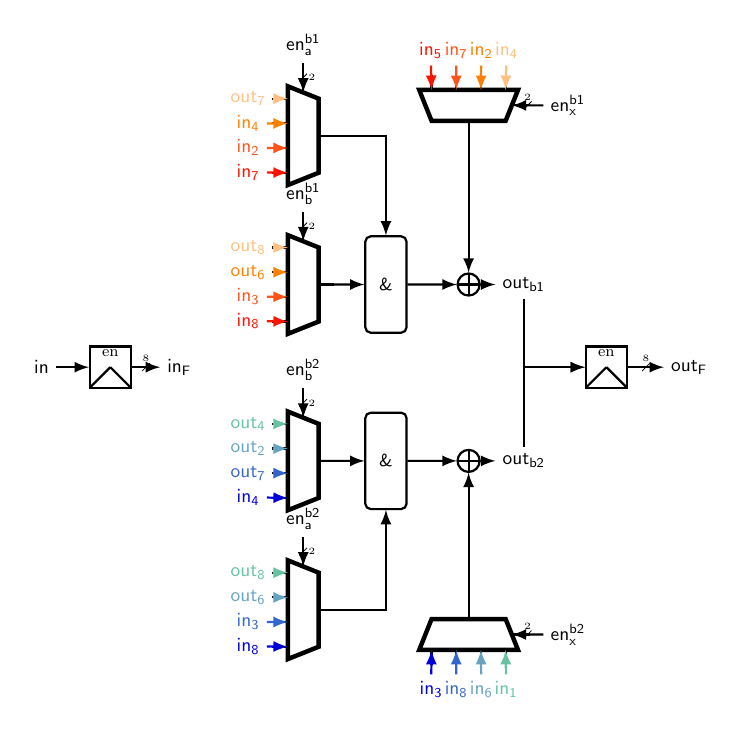
\begin{tikzpicture}[thick]% coordinates%\begin{}[]%\addplot coordinates {};%\end{}%\end{}
\begin{scope}[scale=.7, every node/.style={transform shape}]
  
  \begin{scope}[xshift = -6cm]
    \node [] (in) at (-.25, 0) {$\mathsf{in}$};
    \draw [] (1, 0) \registerEn{reg1};
    \node [] (inf) at (2.25, 0) {$\mathsf{in_{F}}$};
    \draw [-latex] (in) -- (reg1);
    \draw [-latex] (reg1) -- node {\bitwidth} node [bitwidth] {8} (inf);
\end{scope}
\begin{scope}[xshift = 3cm]
  \draw [] (1, 0) \registerEn{reg2};
  \node [] (outf) at (2.5, 0) {$\mathsf{out_{F}}$};
\end{scope}



  \begin{scope}[xshift = -1.5cm]
  
  \node [mux 4by2, thick, yscale=-.8](M1) at (0, 1.5){};
  \node [color = red!85!orange] (in1) at (-1, .84) {$\mathsf{in_8}$};
  \node [color = red!50!orange!90!white] (in2) at (-1, 1.28) {$\mathsf{in_3}$};
  \node [color = orange] (in3) at (-1, 1.72) {$\mathsf{out_6}$};
  \node [color = orange!50!white] (in4) at (-1, 2.17) {$\mathsf{out_8}$};
  \node [] (en1b) at (0, 3.15) {$\mathsf{en_b^{b1}}$};
  \draw [-latex] (en1b) -- node {\bitwidth} node [bitwidthvert] {2}(M1.bbpin 1);

  \draw [-latex, thick, color = red!85!orange] (in1) -- (M1.blpin 1);
  \draw [-latex, thick, color = red!50!orange!90!white] (in2) -- (M1.blpin 2);
  \draw [-latex, thick, color = orange] (in3) -- (M1.blpin 3);
  \draw [-latex, thick, color = orange!50!white] (in4) -- (M1.blpin 4);

\end{scope}

\begin{scope}[xshift = -1.5cm, yshift = 2.7cm]
  \node [mux 4by2, thick, yscale=-.8](M2) at (0, 1.5){};

  \node [color = red!85!orange] (in1) at (-1, .84) {$\mathsf{in_7}$};
  \node [color = red!50!orange!90!white] (in2) at (-1, 1.28) {$\mathsf{in_2}$};
  \node [color = orange] (in3) at (-1, 1.72) {$\mathsf{in_4}$};
  \node [color = orange!50!white] (in4) at (-1, 2.17) {$\mathsf{out_7}$};

  \node [] (en1a) at (0, 3.15) {$\mathsf{en_a^{b1}}$};
  \draw [-latex] (en1a) -- node {\bitwidth} node [bitwidthvert] {2} (M2.bbpin 1);
  \draw [-latex, thick, color = red!85!orange] (in1) -- (M2.blpin 1);
  \draw [-latex, thick, color = red!50!orange!90!white] (in2) -- (M2.blpin 2);
  \draw [-latex, thick, color = orange] (in3) -- (M2.blpin 3);
  \draw [-latex, thick, color = orange!50!white] (in4) -- (M2.blpin 4);
\end{scope}

\begin{scope}[xshift = 1.5cm, yshift = 3.25cm]
  \node [mux 4by2, thick, yscale=-1, xscale = .8, rotate = 90](M3) at (0, 1.5){};

  \node [color = red!85!orange] (in1) at (-.69, 2.5) {$\mathsf{in_5}$};
  \node [color = red!50!orange!90!white] (in2) at (-.225, 2.5) {$\mathsf{in_7}$};
  \node [color = orange] (in3) at (.23, 2.5) {$\mathsf{in_2}$};
  \node [color = orange!50!white] (in4) at (.69, 2.5) {$\mathsf{in_4}$};
  \node [] (en1x) at (1.8, 1.5) {$\mathsf{en_x^{b1}}$};
  \draw [-latex] (en1x) -- node {\bitwidth} node [bitwidth] {2} (M3.bbpin 1);

  \draw [-latex, thick, color = red!85!orange] (in1) -- (M3.blpin 1);
  \draw [-latex, thick, color = red!50!orange!90!white] (in2) -- (M3.blpin 2);
  \draw [-latex, thick, color = orange] (in3) -- (M3.blpin 3);
  \draw [-latex, thick, color = orange!50!white] (in4) -- (M3.blpin 4);
\end{scope}
\begin{scope}[xshift = 1.5cm, yshift = -6.35cm]
  \node [mux 4by2, thick, yscale=1, xscale = .8, rotate = 90](M4) at (0, 1.5){};


  \node [color = blue!85!black] (in1) at (-.68, .5) {$\mathsf{in_3}$};
  \node [color = blue!75!green!80!white] (in2) at (-.225, .5) {$\mathsf{in_8}$};
  \node [color = green!40!blue!60!white] (in3) at (.23, .5) {$\mathsf{in_6}$};
  \node [color = green!60!blue!60!white] (in4) at (.68, .5) {$\mathsf{in_1}$};

  \node [] (en1b) at (1.8, 1.5) {$\mathsf{en_x^{b2}}$};
  \draw [-latex] (en1b) -- node {\bitwidth} node [bitwidth] {2}(M4.bbpin 1);
  \draw [-latex, thick, color = blue!85!black] (in1) -- (M4.blpin 1);
  \draw [-latex, thick, color = blue!75!green!80!white] (in2) -- (M4.blpin 2);
  \draw [-latex, thick, color = green!40!blue!60!white] (in3) -- (M4.blpin 3);
  \draw [-latex, thick, color = green!60!blue!60!white] (in4) -- (M4.blpin 4);
\end{scope}
\begin{scope}[xshift = -1.5cm, yshift = -5.9cm]
  \node [mux 4by2, thick, yscale=-.8](M5) at (0, 1.5){};

  \node [color = blue!85!black] (in1) at (-1, .84) {$\mathsf{in_8}$};
  \node [color = blue!75!green!80!white] (in2) at (-1, 1.28) {$\mathsf{in_3}$};
  \node [color = green!40!blue!60!white] (in3) at (-1, 1.72) {$\mathsf{out_6}$};
  \node [color = green!60!blue!60!white] (in4) at (-1, 2.17) {$\mathsf{out_8}$};
  
  \node [] (en1b) at (0, 3.15) {$\mathsf{en_a^{b2}}$};
  \draw [-latex] (en1b) -- node {\bitwidth} node [bitwidthvert] {2}(M5.bbpin 1);
  \draw [-latex, thick, color = blue!85!black] (in1) -- (M5.blpin 1);
  \draw [-latex, thick, color = blue!75!green!80!white] (in2) -- (M5.blpin 2);
  \draw [-latex, thick, color = green!40!blue!60!white] (in3) -- (M5.blpin 3);
  \draw [-latex, thick, color = green!60!blue!60!white] (in4) -- (M5.blpin 4);
\end{scope}
\begin{scope}[xshift = -1.5cm, yshift = -3.2cm]
  \node [mux 4by2, thick, yscale=-.8](M6) at (0, 1.5){};

  \node [color = blue!85!black] (in1) at (-1, .84) {$\mathsf{in_4}$};
  \node [color = blue!75!green!80!white] (in2) at (-1, 1.28) {$\mathsf{out_7}$};
  \node [color = green!40!blue!60!white] (in3) at (-1, 1.72) {$\mathsf{out_2}$};
  \node [color = green!60!blue!60!white] (in4) at (-1, 2.17) {$\mathsf{out_4}$};
  
  \node [] (en1b) at (0, 3.15) {$\mathsf{en_b^{b2}}$};
  \draw [-latex] (en1b) -- node {\bitwidth} node [bitwidthvert] {2}(M6.bbpin 1);
  \draw [-latex, thick, color = blue!85!black] (in1) -- (M6.blpin 1);
  \draw [-latex, thick, color = blue!75!green!80!white] (in2) -- (M6.blpin 2);
  \draw [-latex, thick, color = green!40!blue!60!white] (in3) -- (M6.blpin 3);
  \draw [-latex, thick, color = green!60!blue!60!white] (in4) -- (M6.blpin 4);
\end{scope}
  \begin{scope}
  
  \node[rectangle,
  minimum width = .75cm,
  minimum height = 1.75cm,
  draw,
  rounded corners = 2pt
  ] (and1) at (0,1.5) {\small \textsf{\&}};

  \node[rectangle,
  minimum width = .75cm,
  minimum height = 1.75cm,
  draw,
  rounded corners = 2pt
  ] (and2) at (0,-1.7) {\small \textsf{\&}};

  \draw [] (1.5, 1.5) \xord{xor1};
  \draw [] (1.5, -1.7) \xord{xor2};
  \node [] (outb1) at (2.5, 1.5) {$\mathsf{out_{b1}}$};
  \node [] (outb2) at (2.5, -1.7) {$\mathsf{out_{b2}}$};
  
\end{scope}

\draw [-latex] (M1.brpin 1) -- (and1);
\draw [-latex] (M6.brpin 1) -- (and2);

\draw [-latex] (M2.brpin 1) -| (and1);
\draw [-latex] (M5.brpin 1) -| (and2);

\draw [-latex] (M3.brpin 1) -| (xor1);
\draw [-latex] (M4.brpin 1) -|  (xor2);

\draw [-latex] (and1) -- (xor1);
\draw [-latex] (and2) -- (xor2);

\draw [-latex] (xor1) -- (outb1);
\draw [-latex] (xor2) -- (outb2);

\draw [-latex] (outb1) |- (reg2);
\draw [-latex] (outb2) |- (reg2);
\draw [-latex] (reg2) -- node {\bitwidth} node [bitwidth] {8} (outf);

\end{scope}

\end{tikzpicture}
    \caption{%
        Architecture of low-latency masked Skinny Sbox.
    }
    \label{fig:sboxopt_circuit}
    \label{fig:sbox}
\end{figure}

Lastly, we discuss fully pipeline architectures.
While such architectures can achieve very high throughput that compensate for
their large area, they are difficult to use in our case.
Indeed, we are not interested in parallel Skinny evaluations (since this is not
useful for encrypting a single message with a Romulus-T leveled
implementation). Therefore, the latency
overhead of filling the pipeline (of at least 6~cycles) is significant when it
is used for only 16 Sbox evaluations (a Skinny round).
We however note that the only other HPC Skinny implementation we
know of uses that strategy, and uses a depth-12 pipeline~\cite{khairallahhardware}.\footnote{%
    Which can be improved to depth-6 thanks to the asymmetric
    latency of HPC2 ANDs.
}

\subsubsection{Skinny.}\label{subsub:skinny}

Based on these Sbox architectures, we design three Skinny implementations with
various area vs. latency trade-offs.
The two first ones are simple round-based architectures, as shown in
\autoref{fig:skinny8}, where either 16~low-latency Sboxes (``low-latency
Skinny'', \skinnyll) or 8~high-throughput (``balanced Skinny'', \skinnyb)
Sboxes are used.
The third implementation (``small Skinny'', \skinnys) targets lower area: it is
a serialized architecture that instantiates only one high-throughput Sbox (that
is used 8~times per round), as shown in \autoref{fig:skinny1}.

\begin{figure}
    \centering
    \resizebox{.9\textwidth}{!}{


%% Document
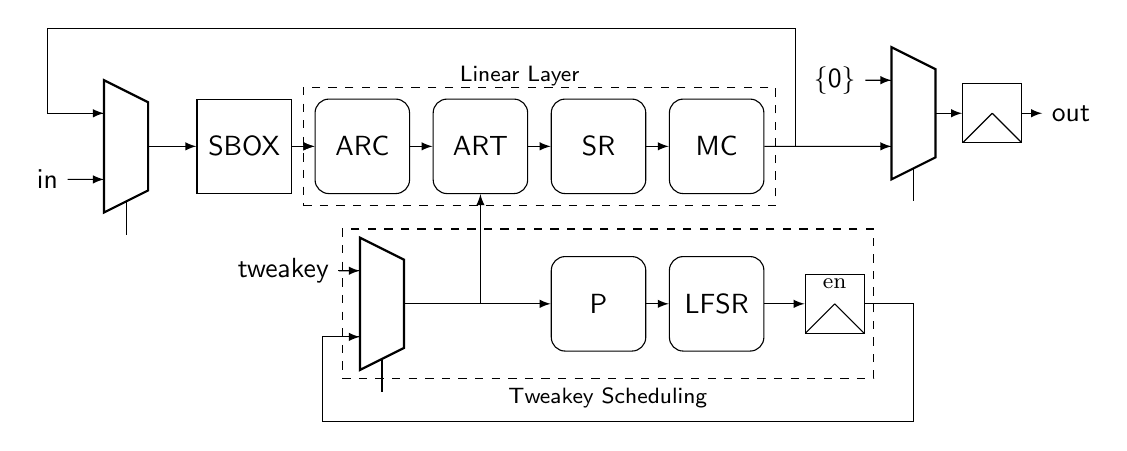
\begin{tikzpicture}[
]
\node [] (i) at (-1, -.42) {$\mathsf{in}$};
\node [] (o) at (12, .42) {$\mathsf{out}$};
\node [] (zero) at (9, .84) {$\mathsf{\{0\}}$};
\node [] (tk) at (2, -1.58) {$\mathsf{tweakey}$};

\node [mux 2by2, rotate = 0](M1) at (0, 0){};
\node [mux 2by2, rotate = 0](M2) at (10, 0.42){};
\node [mux 2by2, rotate = 0](M3) at (3.25, -2){};

\node[rectangle,
minimum width = 1.2cm,
minimum height = 1.2cm,
draw] (B1) at (1.5,0) {\textsf{SBOX}};

\node[rectangle,
minimum width = 1.2cm,
minimum height = 1.2cm,
rounded corners = 5pt,
draw] (arc) at (3,0) {\textsf{ARC}};


\node[rectangle,
minimum width = 1.2cm,
rounded corners = 5pt, 
minimum height = 1.2cm,
draw] (art) at (4.5,0) {\textsf{ART}};
\node [] (ll) at (5, .9) {\footnotesize\textsf{Linear Layer}};

\node[rectangle,
dashed,
minimum width = 6cm,
minimum height = 1.5cm,
draw] (sr) at (5.25,0) {};

\node[rectangle,
minimum width = 1.2cm,
rounded corners = 5pt, 
minimum height = 1.2cm,
draw] (sr) at (6,0) {\textsf{SR}};

\node[rectangle,
minimum width = 1.2cm,
rounded corners = 5pt, 
minimum height = 1.2cm,
draw] (mc) at (7.5,0) {\textsf{MC}};

\node[rectangle,
minimum width = 1.2cm,
rounded corners = 5pt, 
minimum height = 1.2cm,
draw] (P) at (6, -2) {\textsf{P}};

\node[rectangle,
minimum width = 1.2cm,
rounded corners = 5pt, 
minimum height = 1.2cm,
draw] (LFSR) at (7.5,-2) { \textsf{LFSR}};

\draw [] (9, -2) \registerEn{reg1};
\draw [] (11, .42) \register{rego};



\draw [-latex] (B1) -- (arc);
\draw [-latex] (arc) -- (art);
\draw [-latex] (art) -- (sr);
\draw [-latex] (sr) -- (mc);
\draw [-latex] (B1) -- (arc);
\draw [-latex] (mc) -- (M2.blpin 2);
\draw [-latex] (M1.brpin 1) -- (B1);
\draw [] (8.5, 0) |- (-1,1.5);
\draw [-latex] (i) -- (M1.blpin 2);

\draw [-latex] (-1, 1.5) |- (M1.blpin 1);
\draw [-latex] (M2.brpin 1) -- (rego);
\draw [-latex] (rego) -- (o);

\draw [-latex] (M3.brpin 1) -- (P);
\draw [-latex] (P) -- (LFSR);
\draw [-latex] (4.5,-2) -- (art);
\draw [-latex] (LFSR) -- (reg1);

\draw [] (reg1) -- (10, -2);

\draw [] (10, -2) |- (2.5, -3.5);
\draw [-latex] (2.5, -3.5) |- (M3.blpin 2);
\draw [-latex] (tk) -- (M3.blpin 1);

\node[rectangle,
dashed,
minimum width = 6.75cm,
minimum height = 1.9cm,
draw] (sr) at (6.12,-2) {};
\node [] (ll) at (6.12, -3.2) {\footnotesize\textsf{Tweakey Scheduling}};
\draw [-latex] (zero) -- (M2.blpin 1);

\end{tikzpicture}}
    \caption{Round-based masked Skinny architecture (\skinnyll and \skinnyb).}
    \label{fig:skinny8}
\end{figure}

\begin{figure}
    \centering
    \resizebox{.9\textwidth}{!}{


%% Document
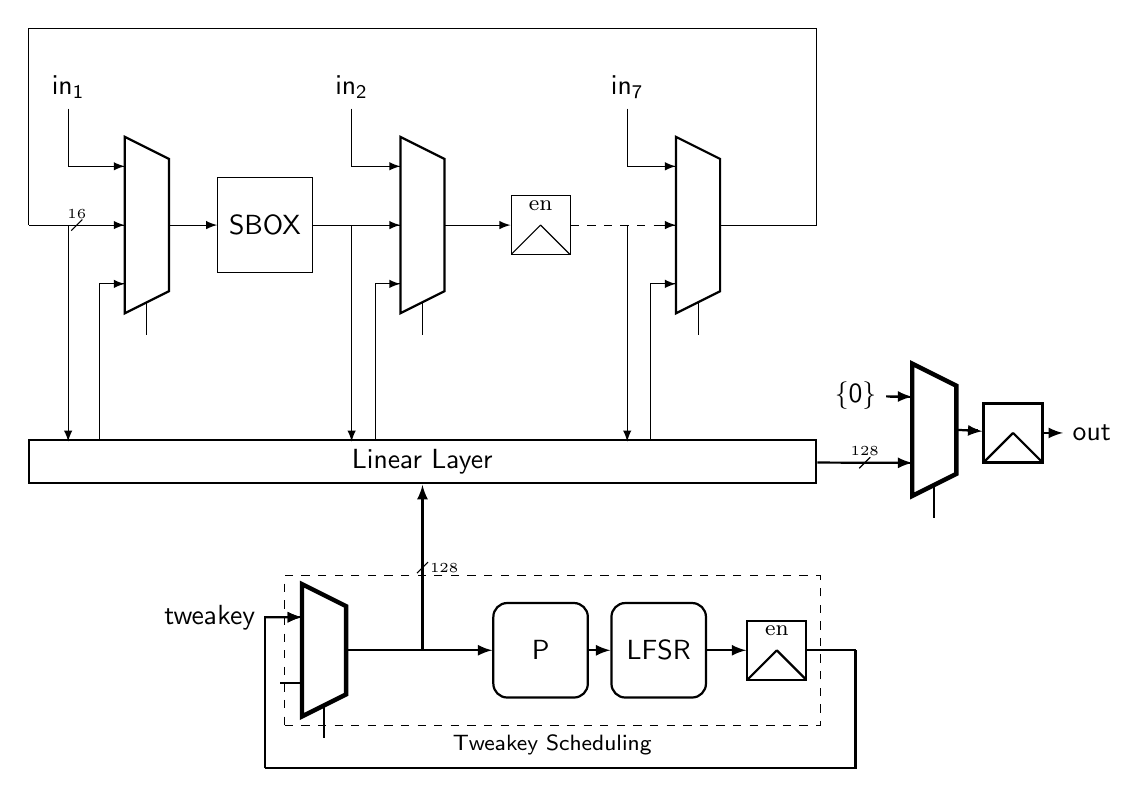
\begin{tikzpicture}[
]
\node [] (i1) at (-1, 1.75) {$\mathsf{in_1}$};
\node [] (i2) at (2.6, 1.75) {$\mathsf{in_2}$};
\node [] (i3) at (6.1, 1.75) {$\mathsf{in_7}$};

\node [mux 3by2, rotate = 0](M1) at (0, 0){};
\node [mux 3by2, rotate = 0](M3) at (3.5, 0){};
\node [mux 3by2, rotate = 0](M2) at (7, 0){};
\node [mux 2by2, rotate = 0, thick](Mo) at (10, -2.6){};


\draw [] (5, 0) \registerEn{reg1};

\node[rectangle,
minimum width = 1.2cm,
minimum height = 1.2cm,
draw] (B1) at (1.5,0) {\textsf{SBOX}};


\node[rectangle,
thick,
minimum width = 10cm,
minimum height = .4cm,
draw] (ll) at (3.5, -3) {\textsf{Linear Layer}};

\draw [-latex] (-1.5,0) -- node {\bitwidth} node [bitwidth] {16} (M1.blpin 2);

\draw [] (M2.brpin 1) -| (8.5, 2.5);
\draw [] (8.5, 2.5) -| (-1.5, 0);
\draw [thick, -latex] (ll) -- node {\bitwidth} node [bitwidth] {128} (Mo.blpin 2);

\draw [-latex] (-1,0) -- (-1, -2.75);
\draw [-latex] (2.6,0) -- (2.6, -2.75);
\draw [-latex] (6.1,0) -- (6.1, -2.75);

\draw [-latex] (-.6,-2.73) |- (M1.blpin 3);
\draw [-latex] (2.9,-2.73) |- (M3.blpin 3);
\draw [-latex] (6.4 ,-2.73) |- (M2.blpin 3);



\draw [-latex] (M1.brpin 1) -- (B1);
\draw [-latex] (B1) -- (M3.blpin 2);
\draw [-latex] (M3.brpin 1) -- (reg1);



\draw [-latex] (i1) |-  (M1.blpin 1);
\draw [-latex] (i2) |- (M3.blpin 1);
\draw [-latex] (i3) |- (M2.blpin 1);

\draw [-latex, dashed] (reg1) -- (M2.blpin 2);


\begin{scope}[yshift = -3.4cm, xshift = -1 cm]
    \node [] (tk) at (1.8, -1.58) {$\mathsf{tweakey}$};
    \draw [thick] (9, -2) \registerEn{reg2};
    \draw [thick] (12, .76) \register{reg3};

    \node [] (o) at (13, .76) {$\mathsf{out}$};
    \node [] (zero) at (10, 1.23) {$\mathsf{\{0\}}$};

    \node [mux 2by2, rotate = 0, thick](M3) at (3.25, -2){};

    \node[rectangle,
    minimum width = 1.2cm,
    minimum height = 1.2cm,
    rounded corners = 5pt,
    thick,
    draw] (P) at (6, -2) {\textsf{P}};

    \node[rectangle,
    minimum width = 1.2cm,
    minimum height = 1.2cm,
    thick,
    rounded corners = 5pt,
    draw] (LFSR) at (7.5,-2) { \textsf{LFSR}};

    \draw [-latex, thick] (M3.brpin 1) -- (P);
    \draw [-latex, thick] (P) -- (LFSR);
    \draw [-latex, thick] (4.5,-2) -- node {\bitwidth} node [bitwidthvert] {128}(4.5, 0.1);
    \draw [-latex, thick] (LFSR) -- (reg2);

    \draw [thick] (reg2) -- (10, -2);
    \draw [thick] (10,-2) |- (2.5, -3.5);
    \draw [-latex, thick] (2.5, -3.5) |- (M3.blpin 1);
    \draw [-latex, thick] (tk) -- (M3.blpin 1);
    \draw [-latex, thick] (zero) -- (Mo.blpin 1);
    \draw [-latex, thick] (reg3) -- (o);
    \draw [-latex, thick] (Mo.brpin 1) -- (reg3);

    \node[rectangle,
    dashed,
    minimum width = 6.8cm,
    minimum height = 1.9cm,
    draw] (sr) at (6.15,-2) {};
    \node [] (ll) at (6.15, -3.2) {\footnotesize\textsf{Tweakey Scheduling}};


\end{scope}

\end{tikzpicture}}
    \caption{Serialized masked Skinny architecture (\skinnys).}
    \label{fig:skinny1}
\end{figure}

Let us now discuss the performance of these implementations.
We consider latency, randomness requirements and area as performance metrics,
since the critical path
will be similar in all cases (it lies in the linear layer).
The latency and maximum randomness requirements per cycle
of the implementations are shown in \autoref{tab:latencyrandomness}.
%\footnote{%
%    This randomness figure characterizes the number of randomness generators
%    needed if no randomness is stored.
%}
We can see that the \skinnys implementation has 8~times the latency of \skinnyb (due to 8x
serialization), while \skinnyll reduces latency by 33~\% compared to \skinnyb.
Regarding randomness, the maximum randomness throughput of \skinnys is 8~times
lower than \skinnyb, and the one of \skinnyll is twice the one of \skinnyb.

\begin{table}
    \centering
    \setlength\tabcolsep{0.4em}
    \begin{tabular}{lcccccc}
        \toprule
       & \multirow{2}{*}{Latency [cycle]} & \multicolumn{5}{c}{Randomness [bit]} \\
       &                          & $d = 2$ & $d=3$   & $d = 4$ & $d=5$   & $d = 6$    \\
       \midrule
        \skinnys  & 2880                     & 2  & 6      & 12   & 20     & 30       \\
        \skinnyb  & 360                      & 16   & 48    & 96 & 160       & 240      \\
        \skinnyll & 240                      & 32       & 96   & 192    & 320  & 480    \\
    \bottomrule
    \end{tabular}
    \vspace*{3ex}
    \caption{
        Skinny-384+ masked implementations: total latency and maximum randomness
        consumption for a single clock cycle (where the total randomness consumption
        is $64 \cdot d \cdot (d-1)$ bits for all three implementations).
    }
    \label{tab:latencyrandomness}
\end{table}

Next, we look at area requirements in \autoref{fig:primarea}.
The Sbox logic area clearly reflects the architectural choices: 2 AND and XOR
gadgets for \skinnys, 16 of each for \skinnyb, and 32 of each for \skinnyll.
Next, the remaining Sbox area is fairly high for \skinnyll due to the large
number of Sbox instances and due to their large MUXes and registers.
For \skinnyb and \skinnys, the larger number MUXes and registers in the Sboxes
of the former compensate for the more complex datapath of the latter, resulting
in a similar ``routing'' area for both of them.
The remaining parts of Skinny are the same for all three architectures.
Overall, the difference in area between the architectures is small for low
number of shares, and increases as the latter grows.
For all considered number of shares ($d \le 6$), the Sboxes do not dominate the
area of neither \skinnys nor \skinnyb, hence \skinnys brings a limited area
gain at a large latency cost compared to \skinnyb.
On the other hand, \skinnyll has an area overhead of up to 39~\% (for $d\le 6$),
and a latency gain of 33~\% over \skinnyb.
\begin{figure}
	\centering
	% This file was created with tikzplotlib v0.9.17.
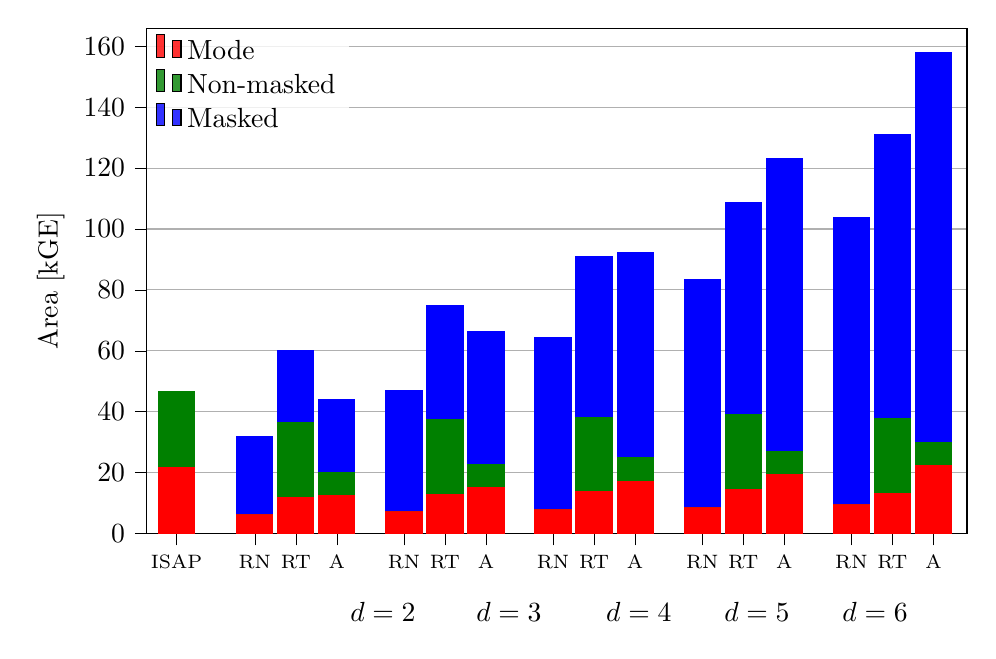
\begin{tikzpicture}

  \node [] (d2) at (3, -1) { $d = 2$};
  \node [] (d3) at (4.6, -1) { $d = 3$};
  \node [] (d4) at (6.25, -1) { $d = 4$};
  \node [] (d5) at (7.75, -1) { $d = 5$};
  \node [] (d6) at (9.25, -1) { $d = 6$};

\begin{axis}[
height=8cm,
legend cell align={left},
legend style={
  draw=none,
  fill opacity=0.8,
  draw opacity=1,
  text opacity=1,
  at={(0.00,1.00)},
  anchor=north west
},
tick align=outside,
tick pos=left,
width=12cm,
x grid style={white!69.0196078431373!black},
xmin=1.0, xmax=6.5,
xtick style={color=black},
xtick={1.2,1.725,2,2.275,2.725,3,3.275,3.725,4,4.275,4.725,5,5.275,5.725,6,6.275},
xticklabel style={rotate=0,font=\scriptsize},
xticklabels={
  ISAP,
  RN,
  RT,
  A,
  RN,
  RT,
  A,  
  RN,
  RT,
  A,
  RN,
  RT,
  A, 
  RN,
  RT,
  A,
},
y grid style={white!69.0196078431373!black},
ylabel={Area [kGE]},
ymajorgrids,
ymin=0, ymax=165.90724575,
ytick style={color=black}
]
\draw[draw=none,fill=red] (axis cs:1.075,0) rectangle (axis cs:1.325,21.9906907142857);
\draw[draw=none,fill=green!50.1960784313725!black] (axis cs:1.075,21.9906907142857) rectangle (axis cs:1.325,46.830795);
\draw[draw=none,fill=red] (axis cs:1.6,0) rectangle (axis cs:1.85,6.58198857142858);
\addlegendimage{ybar,ybar legend,draw=none,fill=red}
\addlegendentry{Mode}

\draw[draw=none,fill=red] (axis cs:1.875,0) rectangle (axis cs:2.125,12.1421064285714);
\draw[draw=none,fill=red] (axis cs:2.15,0) rectangle (axis cs:2.4,12.5364521428571);
\draw[draw=none,fill=red] (axis cs:2.6,0) rectangle (axis cs:2.85,7.29130857142857);
\draw[draw=none,fill=red] (axis cs:2.875,0) rectangle (axis cs:3.125,13.1074792857143);
\draw[draw=none,fill=red] (axis cs:3.15,0) rectangle (axis cs:3.4,15.3762942857143);
\draw[draw=none,fill=red] (axis cs:3.6,0) rectangle (axis cs:3.85,8.108355);
\draw[draw=none,fill=red] (axis cs:3.875,0) rectangle (axis cs:4.125,13.9505428571429);
\draw[draw=none,fill=red] (axis cs:4.15,0) rectangle (axis cs:4.4,17.4141992857143);
\draw[draw=none,fill=red] (axis cs:4.6,0) rectangle (axis cs:4.85,8.86489571428572);
\draw[draw=none,fill=red] (axis cs:4.875,0) rectangle (axis cs:5.125,14.7702007142857);
\draw[draw=none,fill=red] (axis cs:5.15,0) rectangle (axis cs:5.4,19.4334978571429);
\draw[draw=none,fill=red] (axis cs:5.6,0) rectangle (axis cs:5.85,9.70250142857143);
\draw[draw=none,fill=red] (axis cs:5.875,0) rectangle (axis cs:6.125,13.436005);
\draw[draw=none,fill=red] (axis cs:6.15,0) rectangle (axis cs:6.4,22.4762);
\draw[draw=none,fill=green!50.1960784313725!black] (axis cs:1.6,6.58198857142858) rectangle (axis cs:1.85,6.58198857142858);
\addlegendimage{ybar,ybar legend,draw=none,fill=green!50.1960784313725!black}
\addlegendentry{Non-masked}

\draw[draw=none,fill=green!50.1960784313725!black] (axis cs:1.875,12.1421064285714) rectangle (axis cs:2.125,36.61888);
\draw[draw=none,fill=green!50.1960784313725!black] (axis cs:2.15,12.5364521428571) rectangle (axis cs:2.4,20.1325171428571);
\draw[draw=none,fill=green!50.1960784313725!black] (axis cs:2.6,7.29130857142857) rectangle (axis cs:2.85,7.29130857142857);
\draw[draw=none,fill=green!50.1960784313725!black] (axis cs:2.875,13.1074792857143) rectangle (axis cs:3.125,37.5796978571429);
\draw[draw=none,fill=green!50.1960784313725!black] (axis cs:3.15,15.3762942857143) rectangle (axis cs:3.4,22.970895);
\draw[draw=none,fill=green!50.1960784313725!black] (axis cs:3.6,8.108355) rectangle (axis cs:3.85,8.108355);
\draw[draw=none,fill=green!50.1960784313725!black] (axis cs:3.875,13.9505428571429) rectangle (axis cs:4.125,38.31039);
\draw[draw=none,fill=green!50.1960784313725!black] (axis cs:4.15,17.4141992857143) rectangle (axis cs:4.4,25.0102642857143);
\draw[draw=none,fill=green!50.1960784313725!black] (axis cs:4.6,8.86489571428572) rectangle (axis cs:4.85,8.86489571428572);
\draw[draw=none,fill=green!50.1960784313725!black] (axis cs:4.875,14.7702007142857) rectangle (axis cs:5.125,39.2558271428572);
\draw[draw=none,fill=green!50.1960784313725!black] (axis cs:5.15,19.4334978571429) rectangle (axis cs:5.4,27.0280985714286);
\draw[draw=none,fill=green!50.1960784313725!black] (axis cs:5.6,9.70250142857143) rectangle (axis cs:5.85,9.70250142857143);
\draw[draw=none,fill=green!50.1960784313725!black] (axis cs:5.875,13.436005) rectangle (axis cs:6.125,37.9345764285714);
\draw[draw=none,fill=green!50.1960784313725!black] (axis cs:6.15,22.4762) rectangle (axis cs:6.4,30.072265);
\draw[draw=none,fill=blue] (axis cs:1.6,6.58198857142858) rectangle (axis cs:1.85,32.0410328571429);
\addlegendimage{ybar,ybar legend,draw=none,fill=blue}
\addlegendentry{Masked}

\draw[draw=none,fill=blue] (axis cs:1.875,36.61888) rectangle (axis cs:2.125,60.1328478571429);
\draw[draw=none,fill=blue] (axis cs:2.15,20.1325171428571) rectangle (axis cs:2.4,44.29109);
\draw[draw=none,fill=blue] (axis cs:2.6,7.29130857142857) rectangle (axis cs:2.85,47.2232907142857);
\draw[draw=none,fill=blue] (axis cs:2.875,37.5796978571429) rectangle (axis cs:3.125,75.134835);
\draw[draw=none,fill=blue] (axis cs:3.15,22.970895) rectangle (axis cs:3.4,66.4682085714286);
\draw[draw=none,fill=blue] (axis cs:3.6,8.108355) rectangle (axis cs:3.85,64.5575221428572);
\draw[draw=none,fill=blue] (axis cs:3.875,38.31039) rectangle (axis cs:4.125,91.2705657142857);
\draw[draw=none,fill=blue] (axis cs:4.15,25.0102642857143) rectangle (axis cs:4.4,92.6045885714286);
\draw[draw=none,fill=blue] (axis cs:4.6,8.86489571428572) rectangle (axis cs:4.85,83.5610071428572);
\draw[draw=none,fill=blue] (axis cs:4.875,39.2558271428572) rectangle (axis cs:5.125,108.897425714286);
\draw[draw=none,fill=blue] (axis cs:5.15,27.0280985714286) rectangle (axis cs:5.4,123.207260714286);
\draw[draw=none,fill=blue] (axis cs:5.6,9.70250142857143) rectangle (axis cs:5.85,104.053770714286);
\draw[draw=none,fill=blue] (axis cs:5.875,37.9345764285714) rectangle (axis cs:6.125,131.263735714286);
\draw[draw=none,fill=blue] (axis cs:6.15,30.072265) rectangle (axis cs:6.4,158.006900714286);
\end{axis}

\end{tikzpicture}

        \caption{
            Area requirements for the three masked Skinny hardware implementations in a
            \SI{65}{nm} ASIC technology using the HPC2 masking scheme.
        }
        \label{fig:primarea}\vspace*{-1cm}
\end{figure}

\subsection{Implementation of the modes}\label{subsec:modes}



We implemented side-channel protected hardware accelerators for
Romulus-N, Romulus-T, Ascon and ISAP, using the primitives described
in \autoref{tab:prim_latency}.
The Romulus-N implementation is fully masked and uses one
\skinnyll instance.
Next, the implementation of Romulus-T is leveled 
with one masked instance of Skinny (we also used \skinnyll) and four non-masked
Skinny instances (with a round-based architecture).
Similarly, the Ascon implementation is also leveled.
The masked \asconp primitive is based on the HPC2 masking scheme and is
serialized with 16 Sbox instances (each Sbox is a 2-stage pipeline 
performing 4~Sbox evaluations per round)\footnote{%
    This choice is somewhat arbitrary: we took a serialization factor that gives a good
    latency versus area trade-off.
    It also happens to lead to a latency of 6 clock cycles per round, which is
    the same latency as a round of \skinnyll.
},
while the non-masked permutation is round-based (1~cycle per round).
Finally, ISAP uses two instances of the non-masked \asconp primitive.

\begin{table}
    \centering
    \setlength\tabcolsep{0.4em}
    \begin{tabular}{lcccc}
        \toprule
    & \multicolumn{2}{c}{Masked}          & \multicolumn{2}{c}{Non-masked}          \\
    & Latency & Architecture & Latency & Architecture \\
    \midrule
        Skinny-384+  & 240 & \skinnyll          & 40  & round-based             \\
        $\asconp^{6}$  & &                & 6  & round-based              \\
        $\asconp^{12}$ & 72  & serialized 4x           & 12 & round-based              \\
        ISAP RK  &              &  & 152 & round-based \\ \bottomrule
    \end{tabular}
    \vspace*{3ex}
    \caption{
        Primitive implementations used in the AEAD cores: latency
        in clock cycles and architecture for masked and non-masked versions.
    }
    \label{tab:prim_latency}
\end{table}

Let us first discuss the latency of these implementations with
\autoref{fig:modelatency}.
The encryption time of Romulus-N grows very quickly with the message size due
to the need of masking all Skinny calls, which are slow compared to non-masked
calls (as shown in \autoref{tab:prim_latency}).
However, for very short messages, Romulus-N is fairly competitive thanks to its
low number of Skinny calls it that case.
On the other hand, Romulus-T has a larger upfront cost, due to the larger
number of Skinny calls even for short messages, however the mode-level leakage resistance
allows to use non-masked calls for the bulk processing, resulting in
lower latency than Romulus-N for long messages.
Next, Ascon enjoys lower initial latency and long-message latency than Romulus-T.
This is due to the lower number of rounds in $\asconp^{6}$ and $\asconp^{12}$ compared to
Skinny (which has 40 rounds).
Finally, the latency of ISAP is between the one of Ascon and Romulus-T.
Indeed, ISAP's bulk processing is very similar to Ascon's, but uses more rounds
to increase the security margin in presence of leakage.
Moreover, the leakage-resilient PRF of ISAP uses many permutation rounds, which
makes it slower than a masked Ascon for short messages, while still being
faster than Romulus-T.

\begin{figure}
    \centering
    \input{./figures/implem_mode/latency_rel.tex}
    \caption{Encryption latency as a function of the message size.}
    \label{fig:modelatency}
\end{figure}

\begin{figure}
    \centering
    % This file was created with tikzplotlib v0.9.17.
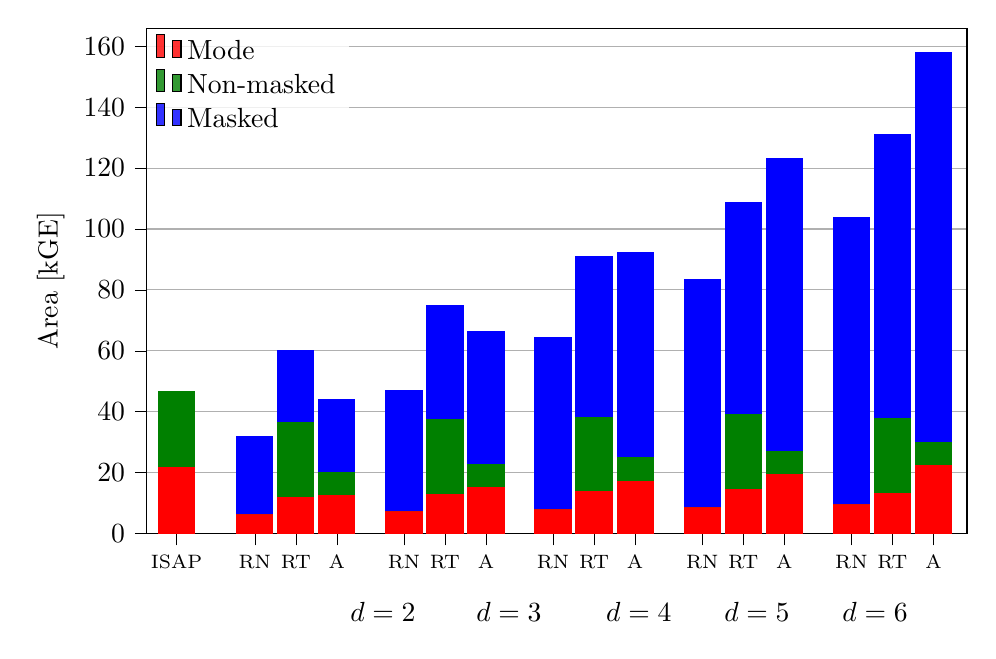
\begin{tikzpicture}

  \node [] (d2) at (3, -1) { $d = 2$};
  \node [] (d3) at (4.6, -1) { $d = 3$};
  \node [] (d4) at (6.25, -1) { $d = 4$};
  \node [] (d5) at (7.75, -1) { $d = 5$};
  \node [] (d6) at (9.25, -1) { $d = 6$};

\begin{axis}[
height=8cm,
legend cell align={left},
legend style={
  draw=none,
  fill opacity=0.8,
  draw opacity=1,
  text opacity=1,
  at={(0.00,1.00)},
  anchor=north west
},
tick align=outside,
tick pos=left,
width=12cm,
x grid style={white!69.0196078431373!black},
xmin=1.0, xmax=6.5,
xtick style={color=black},
xtick={1.2,1.725,2,2.275,2.725,3,3.275,3.725,4,4.275,4.725,5,5.275,5.725,6,6.275},
xticklabel style={rotate=0,font=\scriptsize},
xticklabels={
  ISAP,
  RN,
  RT,
  A,
  RN,
  RT,
  A,  
  RN,
  RT,
  A,
  RN,
  RT,
  A, 
  RN,
  RT,
  A,
},
y grid style={white!69.0196078431373!black},
ylabel={Area [kGE]},
ymajorgrids,
ymin=0, ymax=165.90724575,
ytick style={color=black}
]
\draw[draw=none,fill=red] (axis cs:1.075,0) rectangle (axis cs:1.325,21.9906907142857);
\draw[draw=none,fill=green!50.1960784313725!black] (axis cs:1.075,21.9906907142857) rectangle (axis cs:1.325,46.830795);
\draw[draw=none,fill=red] (axis cs:1.6,0) rectangle (axis cs:1.85,6.58198857142858);
\addlegendimage{ybar,ybar legend,draw=none,fill=red}
\addlegendentry{Mode}

\draw[draw=none,fill=red] (axis cs:1.875,0) rectangle (axis cs:2.125,12.1421064285714);
\draw[draw=none,fill=red] (axis cs:2.15,0) rectangle (axis cs:2.4,12.5364521428571);
\draw[draw=none,fill=red] (axis cs:2.6,0) rectangle (axis cs:2.85,7.29130857142857);
\draw[draw=none,fill=red] (axis cs:2.875,0) rectangle (axis cs:3.125,13.1074792857143);
\draw[draw=none,fill=red] (axis cs:3.15,0) rectangle (axis cs:3.4,15.3762942857143);
\draw[draw=none,fill=red] (axis cs:3.6,0) rectangle (axis cs:3.85,8.108355);
\draw[draw=none,fill=red] (axis cs:3.875,0) rectangle (axis cs:4.125,13.9505428571429);
\draw[draw=none,fill=red] (axis cs:4.15,0) rectangle (axis cs:4.4,17.4141992857143);
\draw[draw=none,fill=red] (axis cs:4.6,0) rectangle (axis cs:4.85,8.86489571428572);
\draw[draw=none,fill=red] (axis cs:4.875,0) rectangle (axis cs:5.125,14.7702007142857);
\draw[draw=none,fill=red] (axis cs:5.15,0) rectangle (axis cs:5.4,19.4334978571429);
\draw[draw=none,fill=red] (axis cs:5.6,0) rectangle (axis cs:5.85,9.70250142857143);
\draw[draw=none,fill=red] (axis cs:5.875,0) rectangle (axis cs:6.125,13.436005);
\draw[draw=none,fill=red] (axis cs:6.15,0) rectangle (axis cs:6.4,22.4762);
\draw[draw=none,fill=green!50.1960784313725!black] (axis cs:1.6,6.58198857142858) rectangle (axis cs:1.85,6.58198857142858);
\addlegendimage{ybar,ybar legend,draw=none,fill=green!50.1960784313725!black}
\addlegendentry{Non-masked}

\draw[draw=none,fill=green!50.1960784313725!black] (axis cs:1.875,12.1421064285714) rectangle (axis cs:2.125,36.61888);
\draw[draw=none,fill=green!50.1960784313725!black] (axis cs:2.15,12.5364521428571) rectangle (axis cs:2.4,20.1325171428571);
\draw[draw=none,fill=green!50.1960784313725!black] (axis cs:2.6,7.29130857142857) rectangle (axis cs:2.85,7.29130857142857);
\draw[draw=none,fill=green!50.1960784313725!black] (axis cs:2.875,13.1074792857143) rectangle (axis cs:3.125,37.5796978571429);
\draw[draw=none,fill=green!50.1960784313725!black] (axis cs:3.15,15.3762942857143) rectangle (axis cs:3.4,22.970895);
\draw[draw=none,fill=green!50.1960784313725!black] (axis cs:3.6,8.108355) rectangle (axis cs:3.85,8.108355);
\draw[draw=none,fill=green!50.1960784313725!black] (axis cs:3.875,13.9505428571429) rectangle (axis cs:4.125,38.31039);
\draw[draw=none,fill=green!50.1960784313725!black] (axis cs:4.15,17.4141992857143) rectangle (axis cs:4.4,25.0102642857143);
\draw[draw=none,fill=green!50.1960784313725!black] (axis cs:4.6,8.86489571428572) rectangle (axis cs:4.85,8.86489571428572);
\draw[draw=none,fill=green!50.1960784313725!black] (axis cs:4.875,14.7702007142857) rectangle (axis cs:5.125,39.2558271428572);
\draw[draw=none,fill=green!50.1960784313725!black] (axis cs:5.15,19.4334978571429) rectangle (axis cs:5.4,27.0280985714286);
\draw[draw=none,fill=green!50.1960784313725!black] (axis cs:5.6,9.70250142857143) rectangle (axis cs:5.85,9.70250142857143);
\draw[draw=none,fill=green!50.1960784313725!black] (axis cs:5.875,13.436005) rectangle (axis cs:6.125,37.9345764285714);
\draw[draw=none,fill=green!50.1960784313725!black] (axis cs:6.15,22.4762) rectangle (axis cs:6.4,30.072265);
\draw[draw=none,fill=blue] (axis cs:1.6,6.58198857142858) rectangle (axis cs:1.85,32.0410328571429);
\addlegendimage{ybar,ybar legend,draw=none,fill=blue}
\addlegendentry{Masked}

\draw[draw=none,fill=blue] (axis cs:1.875,36.61888) rectangle (axis cs:2.125,60.1328478571429);
\draw[draw=none,fill=blue] (axis cs:2.15,20.1325171428571) rectangle (axis cs:2.4,44.29109);
\draw[draw=none,fill=blue] (axis cs:2.6,7.29130857142857) rectangle (axis cs:2.85,47.2232907142857);
\draw[draw=none,fill=blue] (axis cs:2.875,37.5796978571429) rectangle (axis cs:3.125,75.134835);
\draw[draw=none,fill=blue] (axis cs:3.15,22.970895) rectangle (axis cs:3.4,66.4682085714286);
\draw[draw=none,fill=blue] (axis cs:3.6,8.108355) rectangle (axis cs:3.85,64.5575221428572);
\draw[draw=none,fill=blue] (axis cs:3.875,38.31039) rectangle (axis cs:4.125,91.2705657142857);
\draw[draw=none,fill=blue] (axis cs:4.15,25.0102642857143) rectangle (axis cs:4.4,92.6045885714286);
\draw[draw=none,fill=blue] (axis cs:4.6,8.86489571428572) rectangle (axis cs:4.85,83.5610071428572);
\draw[draw=none,fill=blue] (axis cs:4.875,39.2558271428572) rectangle (axis cs:5.125,108.897425714286);
\draw[draw=none,fill=blue] (axis cs:5.15,27.0280985714286) rectangle (axis cs:5.4,123.207260714286);
\draw[draw=none,fill=blue] (axis cs:5.6,9.70250142857143) rectangle (axis cs:5.85,104.053770714286);
\draw[draw=none,fill=blue] (axis cs:5.875,37.9345764285714) rectangle (axis cs:6.125,131.263735714286);
\draw[draw=none,fill=blue] (axis cs:6.15,30.072265) rectangle (axis cs:6.4,158.006900714286);
\end{axis}

\end{tikzpicture}

    \caption{%
        Area requirements of leakage-resistant hardware AEAD cores in
        \SI{65}{nm} ASIC technology.
        For leveled implementations, the area is split in three part:
        DPA-protected (i.e., masked) primitives, SPA-protected primitives (implemented in parallel), and mode (i.e., logic not in a primitive).
				RN/RT respectively stand for Romulus-N/Romulus-T and A stands for Ascon.
    }
    \label{fig:modearea}
\end{figure}


Let us now discuss the area usage with \autoref{fig:modearea}.
As a general trend, for implementations with a masked primitive, the area for
that primitive dominates the overall area, with the exception of Romulus-T with
$d=2$ shares (where the area of the four non-masked Skinny instances dominates).
These results therefore confirms the interest of leveled implementations.
Next, the areas for all these modes is fairly similar, with a slight advantage
to Ascon and Romulus-N at $d=2,3$ shares thanks to their lower unmasked area, while
Romulus-T and Romulus-N are a bit better than Ascon for larger numbers of
shares, thanks to using less masked AND gadgets.
Lastly, the area for ISAP is similar to the area of the leveled implementations
with $d=2$ shares.

\section{Conclusion}

Even though the previous quantitative results should be interpreted with care, since
they explore only a few points in the design space (e.g., we considered only
round-based architectures for non-masked primitives and did not optimize the
masking randomness usage), their comparison highlights a few general trends.

\smallskip

First, for long messages, leveled implementations bring large latency
improvements while their area overheads remain small over non-leveled
implementations. This is because unmasked primitives are small compared to the masked
ones, especially when the number of shares is large.
This smaller unmasked area as well as lower latency naturally translate
into large energy savings.
The candidates that can be implemented in such a way for both
encryption and decryption (grade-2 and grade-3, see
\autoref{tab:modes_grades}) will benefit most from these savings.
However, having such mode-level characteristics usually implies more complex
modes of operations, which leads to worse performance for small messages, as
shown by the comparison between Romulus-N and the grade-2/grade-3 candidates.

\begin{table}
    \centering
    \setlength\tabcolsep{0.0em}
    \begin{tabular}{c@{\hspace{1.0em}}c@{\hspace{1.0em}}c}
        \toprule
        Grade & Security & Candidates \\
        \midrule
        0 & CCA+CI & Elephant, GIFT-COFB, Romulus-M/N, TinyJambu \\
        1 & CCAL1+CIL1 & PHOTON-Beetle, Sparkle, Xoodyak \\
        2 & CCAmL1+CIML2 & Ascon \\
        3 & CCAmL2+CIML2 & ISAP, Romulus-T \\
        \bottomrule
    \end{tabular}
    \vspace*{3ex}
    \caption{
        NIST LWC finalists grouped by mode-level leakage resistance.
    }
    \label{tab:modes_grades}\vspace*{-0.5cm}
\end{table}

Second, the leakage-resilient PRF technique used by ISAP leads to low area
implementation (similar to a leveled implementations with two shares), and
its latency is comparable to leveled implementations.
Such techniques therefore appear quite promising in hardware implementation
setting. Yet, we note that on the side-channel security side, the formal security 
guarantees of such implementations have been much less analyzed than masking
and their practical security evaluation can be more challenging as well (see, e.g.,~\cite{DBLP:conf/cosade/UdvarhelyiBS21}).


Finally, we observe that the different security margins of the algorithms we implemented
can explain some of the observed performance differences.
For example, the differences in latency between the leveled implementations of
Ascon and ISAP are explained by their number of rounds: the hashing part of ISAP
uses $\asconp^{12}$ while the Ascon inner sponge part uses only $\asconp^{6}$.
When considering CIML2, both should however withstand the same attacks.

Overall, these results backup our suggestion that
from a side-channel security viewpoint, 
the finalists of the NIST's Lightweight Crypto competition differ more 
by their qualitative features than by their quantitative performances.

%Finally qualitative properties are not free (CCAmL2, permutation vs TBC,
%flexibility w.r.t. SCA protection), so that's more the question than pure best
%performance.
%
%
%future work SW

\medskip

\noindent\textbf{Acknowledgments.} Ga\"{e}tan Cassiers and Fran\c{c}ois-Xavier Standaert are respectively
Research Fellow and Senior Associate Researcher of the Belgian Fund for Scientific
Research (FNRS-F.R.S.). This work has been funded in part by the ERC consolidator grant 
number 724725 (acronym SWORD), by the Walloon region CyberExcellence project number 2110186 (acronym Cyberwal) and by the Horizon Europe project 1010706275 (acronym REWIRE).


\bibliographystyle{alpha}
\bibliography{refs}

\end{document}
